\documentclass[12pt,a4paper]{article}

% ─── Encodage & Langue ─────────────────────────────────────────────
\usepackage[utf8]{inputenc}
\usepackage[T1]{fontenc}
\usepackage[french]{babel}
\usepackage{lmodern}
\usepackage{textcomp}

% ─── Mathématiques ─────────────────────────────────────────────────
\usepackage{amsmath, amssymb, amsthm}

% ─── Mise en page ──────────────────────────────────────────────────
\usepackage{geometry}
\geometry{hmargin=2.5cm, vmargin=3cm}
\usepackage{setspace}
\setstretch{1.2}

% ─── Couleurs ──────────────────────────────────────────────────────
\usepackage[table]{xcolor}
\definecolor{SectionColor}{RGB}{0,76,153}
\definecolor{SubsectionColor}{RGB}{0,76,153}
\definecolor{SubsubsectionColor}{RGB}{0,102,204}
\definecolor{cryptoBlue}{RGB}{0,102,204}
\definecolor{MarsaBlue}{RGB}{11,43,94}
\definecolor{MarsaOrange}{RGB}{230,81,0}
\definecolor{CodeBg}{RGB}{245,245,250}
\definecolor{TableHeader}{RGB}{11,43,94}

% ─── Titres ────────────────────────────────────────────────────────
\usepackage{titlesec}
\titleformat{\section}
  {\color{SectionColor}\normalfont\Large\bfseries}{\thesection}{1em}{}
\titleformat{\subsection}
  {\color{SubsectionColor}\normalfont\large\bfseries}{\thesubsection}{1em}{}
\titleformat{\subsubsection}
  {\color{SubsubsectionColor}\normalfont\normalsize\bfseries}{\thesubsubsection}{1em}{}

% ─── Tableaux ──────────────────────────────────────────────────────
\usepackage{array}
\usepackage{booktabs}
\usepackage{float}
\usepackage{caption}
\usepackage{multirow}
\usepackage{longtable}

% ─── Listes ────────────────────────────────────────────────────────
\usepackage{enumitem}
\setlist[itemize,1]{
  leftmargin=1cm,
  label=\textbullet,
  labelsep=0.6em,
  itemsep=0.2em,
  topsep=0.3em,
  parsep=0pt
}

% ─── Boîtes & Cadres ───────────────────────────────────────────────
\usepackage{tcolorbox}
\tcbuselibrary{skins, listings}

% Definition d'une couleur sombre pour le code (VS Code dark style)
\definecolor{VSCodeDark}{RGB}{30,30,30}
\definecolor{VSCodeHeader}{RGB}{45,45,45}
\definecolor{VSCodeText}{RGB}{220,220,220}
\definecolor{VSCodeKeyword}{RGB}{86,156,214}
\definecolor{VSCodeString}{RGB}{206,145,120}
\definecolor{VSCodeComment}{RGB}{106,153,85}
\definecolor{VSCodeNumber}{RGB}{181,206,168}

\newtcblisting{vscodeWindow}[2][]{
  enhanced,
  colback=VSCodeDark,
  colframe=VSCodeHeader,
  colupper=VSCodeText,
  arc=6pt,
  boxrule=1.5pt,
  title={\quad\quad\quad \texttt{#2}},
  coltitle=white,
  fonttitle=\bfseries\small,
  attach boxed title to top left={yshift=-2.2mm, xshift=12mm},
  boxed title style={colback=VSCodeDark, colframe=VSCodeHeader, arc=3pt},
  overlay={
    % Three buttons (red, yellow, green) simulating macOS/VS Code controls
    \fill[red!80!black] ([xshift=10pt, yshift=-8pt]frame.north west) circle (4pt);
    \fill[yellow!80!black] ([xshift=22pt, yshift=-8pt]frame.north west) circle (4pt);
    \fill[green!80!black] ([xshift=34pt, yshift=-8pt]frame.north west) circle (4pt);
  },
  listing only,
  listing engine=listings,
  listing options={
    language=Python,
    inputencoding=utf8,
    backgroundcolor=\color{VSCodeDark},
    basicstyle=\ttfamily\footnotesize\color{VSCodeText},
    keywordstyle=\color{VSCodeKeyword}\bfseries,
    stringstyle=\color{VSCodeString},
    commentstyle=\color{VSCodeComment}\itshape,
    numberstyle=\tiny\color{gray},
    numbers=left,
    stepnumber=1,
    numbersep=8pt,
    xleftmargin=17pt,
    xrightmargin=5pt,
    breaklines=true,
    breakatwhitespace=false,
    tabsize=4,
    showstringspaces=false,
    upquote=true,
    columns=flexible,
    keepspaces=true,
    literate=
      {é}{{\'{e}}}1 {è}{{\`{e}}}1 {ê}{{\^{e}}}1 {ë}{{\"{e}}}1
      {à}{{\`{a}}}1 {â}{{\^{a}}}1 {ä}{{\"{a}}}1
      {î}{{\^{i}}}1 {ï}{{\"{i}}}1
      {ô}{{\^{o}}}1 {ö}{{\"{o}}}1
      {ù}{{\`{u}}}1 {û}{{\^{u}}}1 {ü}{{\"{u}}}1
      {ç}{{\c{c}}}1
      {É}{{\'{E}}}1 {È}{{\`{E}}}1 {Ê}{{\^{E}}}1
      {À}{{\`{A}}}1 {Â}{{\^{A}}}1
      {Î}{{\^{I}}}1 {Ï}{{\"{I}}}1
      {Ô}{{\^{O}}}1
      {Ù}{{\`{U}}}1 {Û}{{\^{U}}}1 {Ü}{{\"{U}}}1
      {œ}{{\oe}}1 {Œ}{{\OE}}1
      {'}{{'}}1 {"}{``}1 {"}{''}}1
  },
  #1
}

\newtcolorbox{explainbox}[1][]{
  enhanced,
  colback=MarsaOrange!5,
  colframe=MarsaOrange!80!black,
  arc=4pt, boxrule=1pt,
  fonttitle=\bfseries,
  coltitle=white,
  #1
}

% ─── Graphiques & Hyperliens ───────────────────────────────────────
\usepackage{graphicx}
\usepackage{url}
\usepackage{hyperref}
\hypersetup{
  colorlinks=true,
  linkcolor=blue!60!black,
  urlcolor=blue!60!black,
  citecolor=blue!60!black
}

% ─── Théorèmes ─────────────────────────────────────────────────────
\newtheorem{definition}{Définition}
\newtheorem{propriete}{Propriété}
\newtheorem{loi}{Loi}
\newtheorem{expert}{Expert}

% ─── Abréviations ──────────────────────────────────────────────────
\usepackage[withpage]{acronym}
\renewcommand{\acsfont}[1]{\textbf{#1}}

% ─── En-têtes / Pieds de page ──────────────────────────────────────
\usepackage{fancyhdr}
\pagestyle{fancy}
\fancyhf{}
\lhead{\textbf{Département des technologies nouvelles -- FPB}}
\rhead{\textbf{Master en D3SI}}
\cfoot{\thepage}
\renewcommand{\headrulewidth}{0.4pt}

% ═══════════════════════════════════════════════════════════════════
\begin{document}
\newgeometry{hmargin=2cm, top=1.5cm, bottom=1.5cm}
\begin{titlepage}
\begin{center}

\begin{tabular}{m{0.25\textwidth} m{0.45\textwidth} m{0.25\textwidth}}
  \centering
\includegraphics[height=2.5cm]{universite.png} &
  \centering
  \begin{minipage}{\linewidth}
    \centering
    \text{\small Université Sultan Moulay Slimane}\\[2pt]
    \text{\small Faculté Polydisciplinaire de Béni Mellal}\\[4pt]
    \text{Département des technologies nouvelles}
  \end{minipage} &
  \centering
\includegraphics[height=2.5cm]{faculte.jpg}
\end{tabular}

\vspace{3mm}
\rule{\linewidth}{0.8pt}
\vspace{8mm}

{\Large \textsc{Projet de Fin d'Études}}\\[0.3cm]
{\small Présenté pour l'obtention du diplôme de}\\[0.2cm]
{\large \textbf{Master en Data Science et Sécurité des Systèmes d'Information}}\\[0.6cm]

\begin{tcolorbox}[
  colframe=SectionColor, colback=white,
  arc=0pt, boxrule=1.5pt,
  center title
]
  \centering\Large\bfseries\color{SectionColor}
  Solution Intelligente de Vision par Ordinateur\\
  et d'Optimisation Logistique Portuaire\\[4pt]
  \normalsize\color{MarsaOrange}
  Automatisation de la Gestion des Conteneurs par IA\\
  pour Marsa Maroc
\end{tcolorbox}

\vspace{0.6cm}

\begin{minipage}[t]{0.45\textwidth}
  \flushleft
  \textbf{Présenté par :}\\[4pt]
  M. \textbf{Fajri Youssef}
\end{minipage}
\hfill
\begin{minipage}[t]{0.45\textwidth}
  \flushright
  \textbf{Sous la direction de :}\\[4pt]
  Pr. \textbf{Ismail Kich}
\end{minipage}

\vspace{0.5cm}

\begin{tcolorbox}[
  colback=gray!5, colframe=gray!30,
  arc=5pt, boxrule=0.5pt
]
  \begin{minipage}[c]{0.70\textwidth}
    \flushleft
    \textbf{Organisme d'accueil :} \textsc{Marsa Maroc}\\[4pt]
    \textit{Encadrant Professionnel : M. Mohamed Qodsi}
  \end{minipage}
\end{tcolorbox}

\vspace{0.3cm}
\begin{center}
  
\includegraphics[height=1.5cm]{repport.png}
\end{center}

\vspace{0.5cm}

\vfill

\rule{0.3\linewidth}{0.5pt}\\[0.2cm]
{\small Faculté Polydisciplinaire -- Université Sultan Moulay Slimane\\
Mghila BP\,: 592 Beni Mellal\quad
Tél\,: +212\,(0)\,523\,42\,46\,85/16\quad
Fax\,: +212\,(0)\,523\,42\,45\,9}\\[4pt]
{\small Année Universitaire : 2025 -- 2026}

\end{center}
\end{titlepage}
\restoregeometry  

% ═══════════════════════════════════════════════════════════════════
% DÉDICACES
% ═══════════════════════════════════════════════════════════════════
\clearpage
\thispagestyle{empty}
\vspace*{5cm}
\begin{center}
  {\Large\itshape Dédicaces}\\[2cm]
  {\large\itshape
  À mes chers parents, pour leur amour inconditionnel et leur soutien constant,\\
  À toute ma famille, pour sa présence et ses encouragements précieux,\\
  À mes amis et collègues de promotion, avec qui j'ai partagé des moments inoubliables,\\
  À tous ceux qui m'ont soutenu tout au long de ce parcours universitaire.}
\end{center}
\vfill

% ═══════════════════════════════════════════════════════════════════
% REMERCIEMENTS
% ═══════════════════════════════════════════════════════════════════
\clearpage
\section*{Remerciements}
\addcontentsline{toc}{section}{Remerciements}

Avant d'entamer ce rapport, je tiens à exprimer ma profonde gratitude et mes sincères remerciements à toutes les personnes qui ont contribué, de près ou de loin, à l'aboutissement de ce projet de fin d'études.

Je remercie tout d'abord \textbf{mon encadrant académique}, Pr. Ismail Kich, professeur à la Faculté Polydisciplinaire de Béni Mellal, pour sa disponibilité, ses précieux conseils, sa rigueur scientifique et son accompagnement bienveillant tout au long de ce travail de recherche et de développement.

Je tiens également à exprimer ma reconnaissance envers \textbf{mon encadrant professionnel}, M. Mohamed Qodsi, au sein de l'organisme d'accueil \textbf{Marsa Maroc}, pour m'avoir accueilli au sein de son équipe technique, pour sa confiance, ses explications détaillées des processus portuaires et ses orientations opérationnelles tout au long du stage.

Mes remerciements s'adressent aussi aux membres du jury qui ont accepté d'examiner et d'évaluer ce travail de fin d'études, m'honorant ainsi de leur jugement précieux.

Enfin, je tiens à exprimer ma gratitude envers l'ensemble du corps professoral du \textbf{Master Data Science et Sécurité des Systèmes d'Information (D3SI)} de la Faculté Polydisciplinaire de Béni Mellal pour la qualité de la formation théorique et pratique qui m'a permis d'aborder ce projet avec sérénité et compétences.

% ═══════════════════════════════════════════════════════════════════
% RÉSUMÉ / ABSTRACT
% ═══════════════════════════════════════════════════════════════════
\clearpage
\section*{Résumé / Abstract}
\addcontentsline{toc}{section}{Résumé / Abstract}

\begin{tcolorbox}[colframe=MarsaBlue, colback=white, title=\textbf{Résumé (Français)}, arc=4pt]
Le présent Projet de Fin d'Études porte sur la conception et le développement d'une plateforme intelligente intégrée combinant la vision par ordinateur et la recherche opérationnelle pour automatiser et optimiser la logistique des conteneurs au sein des terminaux portuaires de Marsa Maroc. La chaîne de traitement développée s'appuie sur le modèle de deep learning YOLOv8 pour la localisation des conteneurs, couplé à un pipeline OCR adaptatif (EasyOCR et algorithme Segment-and-Stitch) pour l'extraction automatique des identifiants normés ISO 6346. Afin d'assurer un traitement vidéo fluide et résilient, une architecture d'ingestion en temps réel basée sur Apache Kafka et un mécanisme de contre-pression (backpressure) est mise en œuvre. Côté logistique, l'allocation spatiale des conteneurs dans le parc de stockage (\textit{yard}) est optimisée via une métaheuristique du Recuit Simulé guidée par la règle de l'échéance la plus proche (EDD -- Earliest Due Date), permettant de minimiser les opérations improductives de double manipulation (\textit{re-handling}). La solution propose également un tableau de bord interactif sous Streamlit intégrant un jumeau numérique 3D en Three.js et la génération automatique de synthèses PDF enrichies par un modèle de langage (LLM). Les évaluations expérimentales démontrent un taux de réussite OCR de 85\,\% et une réduction de plus de 75\,\% du taux de \textit{re-handling}.
\\[6pt]
\textbf{Mots-clés :} Vision par Ordinateur, Reconnaissance Optique de Caractères (OCR), Optimisation Logistique Portuaire, Recuit Simulé, Streaming Temps Réel.
\end{tcolorbox}

\vspace{0.8cm}

\begin{tcolorbox}[colframe=SectionColor, colback=white, title=\textbf{Abstract (English)}, arc=4pt]
This Master's thesis focuses on the design and development of an integrated intelligent platform combining computer vision and operations research to automate and optimize container terminal logistics for Marsa Maroc. The developed pipeline leverages the YOLOv8 deep learning architecture for real-time container detection, paired with an adaptive OCR pipeline (EasyOCR and the Segment-and-Stitch algorithm) for automated ISO 6346 code recognition. To ensure scalable and fault-tolerant video processing, an asynchronous streaming infrastructure using Apache Kafka with backpressure management is deployed. On the yard management side, spatial allocation of containers is optimized using a Simulated Annealing metaheuristic governed by the Earliest Due Date (EDD) dispatching rule, drastically reducing unproductive re-handling operations. Additionally, the system provides an interactive Streamlit dashboard featuring a 3D virtual yard digital twin powered by Three.js and automated PDF reporting augmented by a Large Language Model (LLM). Experimental results demonstrate an overall OCR accuracy of 85\% and a reduction of over 75\% in re-handling rates under high yard occupancy.
\\[6pt]
\textbf{Keywords:} Computer Vision, Optical Character Recognition (OCR), Port Logistics Optimization, Simulated Annealing, Real-Time Streaming.
\end{tcolorbox}

% ═══════════════════════════════════════════════════════════════════
% TABLE DES MATIÈRES
% ═══════════════════════════════════════════════════════════════════
\clearpage
\pagenumbering{roman}
\setcounter{page}{1}

\tableofcontents
\newpage

\listoffigures
\addcontentsline{toc}{section}{Liste des figures}
\newpage

\listoftables
\addcontentsline{toc}{section}{Liste des tableaux}
\newpage

% ═══════════════════════════════════════════════════════════════════
% LISTE DES ABRÉVIATIONS
% ═══════════════════════════════════════════════════════════════════
\section*{Liste des abréviations}
\addcontentsline{toc}{section}{Liste des abréviations}
\begin{acronym}[CLAHE]
  \acro{PFE}{Projet de Fin d'Études}
  \acro{D3SI}{Data Science et Sécurité des Systèmes d'Information}
  \acro{IA}{Intelligence Artificielle}
  \acro{OCR}{Optical Character Recognition}
  \acro{CNN}{Convolutional Neural Network}
  \acro{YOLO}{You Only Look Once}
  \acro{STS}{Ship-to-Shore}
  \acro{RTG}{Rubber Tyred Gantry}
  \acro{TEU}{Twenty-foot Equivalent Unit}
  \acro{EDD}{Earliest Due Date}
  \acro{SA}{Simulated Annealing}
  \acro{API}{Application Programming Interface}
  \acro{REST}{Representational State Transfer}
  \acro{ORM}{Object-Relational Mapping}
  \acro{LLM}{Large Language Model}
  \acro{IoT}{Internet of Things}
  \acro{ISO}{International Organization for Standardization}
  \acro{CLAHE}{Contrast Limited Adaptive Histogram Equalization}
  \acro{KPI}{Key Performance Indicator}
  \acro{PDF}{Portable Document Format}
  \acro{SQL}{Structured Query Language}
  \acro{OSD}{Orientation and Script Detection}
  \acro{CRAFT}{Character Region Awareness for Text Detection}
  \acro{CRNN}{Convolutional Recurrent Neural Network}
  \acro{CTC}{Connectionist Temporal Classification}
  \acro{SWOT}{Strengths, Weaknesses, Opportunities, Threats}
  \acro{CRP}{Container Relocation Problem}
  \acro{YSP}{Yard Stacking Problem}
  \acro{TOS}{Terminal Operating System}
\end{acronym}

% ═══════════════════════════════════════════════════════════════════
% CORPS DU DOCUMENT
% ═══════════════════════════════════════════════════════════════════
\newpage
\pagenumbering{arabic}
\setcounter{page}{1}

% ─────────────────────────────────────────────────────────────────
% INTRODUCTION GÉNÉRALE
% ─────────────────────────────────────────────────────────────────
\section*{Introduction Générale}
\addcontentsline{toc}{section}{Introduction Générale}

Le commerce international moderne repose intrinsèquement sur la fluidité des flux logistiques maritimes. En effet, plus de 80\,\% des échanges mondiaux de marchandises s'effectuent par voie maritime, et la majorité de ces marchandises est transportée dans des conteneurs standardisés \cite{ISO6346}. Face à cette massification des flux, l'efficacité des infrastructures portuaires est devenue un facteur clé de la compétitivité économique des nations. L'introduction des technologies numériques et des systèmes d'intelligence artificielle au sein des terminaux portuaires est aujourd'hui indispensable pour accélérer les opérations et garantir une traçabilité sans faille \cite{Kim2002}.

Au Maroc, \textbf{Marsa Maroc} s'affirme comme le leader incontesté de l'exploitation de terminaux portuaires. L'entreprise gère des millions d'unités d'équivalent vingt pieds (EVP) chaque année. Cependant, malgré la modernisation constante des infrastructures matérielles (portiques géants, grues de parc automatisées), le suivi logistique et l'allocation spatiale des conteneurs au sein des terminaux reposent encore en partie sur des interventions humaines manuelles.

Lors du déchargement d'un porte-conteneurs par les portiques \ac{STS}, l'identification des codes ISO 6346 des conteneurs est effectuée visuellement par les opérateurs ou par des agents au sol qui saisissent manuellement les codes dans le système. Ce processus, bien que rodé, présente d'importantes faiblesses :
\begin{itemize}
  \item Il est sujet à des erreurs de lecture humaine, accentuées par la fatigue, la nuit ou des conditions climatiques défavorables\,;
  \item Il génère des goulots d'étranglement qui ralentissent le rythme de déchargement des grues \ac{STS}\,;
  \item Il manque d'immédiateté et de synchronisation temps réel avec le système d'ordonnancement du parc de stockage (\textit{yard}).
\end{itemize}

De plus, le positionnement physique des conteneurs dans le parc constitue un problème d'optimisation complexe. Une mauvaise planification spatiale entraîne le phénomène coûteux du \textit{shuffling} ou \textit{re-handling} (doubles manipulations) \cite{Caserta2011, Jin2015}. Ce cas se présente lorsqu'un conteneur situé au bas d'une pile doit être chargé en priorité sur un camion alors que d'autres conteneurs sont empilés au-dessus de lui, obligeant la grue de parc \ac{RTG} à déplacer inutilement les conteneurs supérieurs.

Ce \ac{PFE} propose d'y remédier en concevant et développant une \textbf{plateforme intelligente intégrée} combinant vision par ordinateur et recherche opérationnelle pour automatiser et optimiser la logistique de Marsa Maroc. La solution développée s'articule autour de plusieurs composants clés :
\begin{enumerate}
  \item Une détection en temps réel par deep learning (\textbf{YOLOv8}) \cite{Redmon2016, Ultralytics} pour localiser les conteneurs et isoler leurs plaques d'immatriculation\,;
  \item Un pipeline de lecture optique de caractères robuste (\textbf{EasyOCR}) \cite{Baek2019CRAFT, Shi2016CRNN} capable de décoder les codes ISO 6346 disposés verticalement ou horizontalement sur les parois des conteneurs\,;
  \item Une infrastructure de streaming asynchrone (\textbf{Apache Kafka}) \cite{Kafka} garantissant la transmission en temps réel des frames de caméras de surveillance vers les modèles d'IA\,;
  \item Un moteur d'optimisation du positionnement combinant la règle de l'échéance la plus proche (\textbf{EDD} -- Earliest Due Date) \cite{Baker2009} et la métaheuristique du \textbf{Recuit Simulé} \cite{Kirkpatrick1983} pour éliminer les doubles manipulations\,;
  \item Un tableau de bord interactif en temps réel sous \textbf{Streamlit} proposant une interface de supervision 3D développée avec \textbf{Three.js} pour représenter virtuellement le parc de conteneurs\,;
  \item Un module de rédaction automatisée de synthèses logistiques alimenté par un modèle de langage (\textbf{LLM}) et exportable sous forme de rapports \textbf{PDF} professionnels.
\end{enumerate}

Le présent rapport est structuré de la manière suivante. Le premier chapitre définit le contexte général, présente l'organisme d'accueil et détaille la problématique opérationnelle ainsi que les spécifications des besoins. Le deuxième chapitre expose l'état de l'art technologique et théorique couvrant le deep learning, l'OCR (avec une explication de CRAFT, CRNN et CTC), le streaming distribué, l'optimisation combinatoire et une étude comparative des travaux connexes récents. Le troisième chapitre présente la conception globale du système et son architecture microservices. Le quatrième chapitre fournit les détails d'implémentation et de développement en exposant la logique des modules clés ainsi que la démonstration fonctionnelle des interfaces applicatives. Le cinquième chapitre présente les résultats expérimentaux, l'évaluation quantitative des performances et l'analyse de la simulation de charge du parc. Enfin, le sixième chapitre dresse un bilan de ce projet et présente les perspectives d'évolutions futures pour l'exploitation portuaire.

\newpage

% ═══════════════════════════════════════════════════════════════════
% CHAPITRE 1 — CONTEXTE GÉNÉRAL
% ═══════════════════════════════════════════════════════════════════
\section{Contexte Général et Présentation du Projet}

Ce premier chapitre pose les bases de notre étude en présentant l'organisme d'accueil, Marsa Maroc, et en décrivant le fonctionnement opérationnel des terminaux portuaires. Nous y détaillons la problématique du traitement manuel des conteneurs ainsi que les objectifs stratégiques et fonctionnels fixés pour la solution technologique proposée.

\subsection{Présentation de l'Organisme d'Accueil : Marsa Maroc}

Créée en décembre 2006 à la suite de la réforme portuaire nationale introduite par la loi 15-02, \textbf{Marsa Maroc} (Société d'Exploitation des Ports) est le concessionnaire historique et l'opérateur logistique leader au Maroc. L'entreprise est en charge de la gestion et de la maintenance de terminaux portuaires dans 9 ports d'importance stratégique le long des côtes atlantique et méditerranéenne du Royaume : Tanger Med, Nador, Al Hoceima, Kénitra, Casablanca, Jorf Lasfar, Safi, Agadir et Laâyoune.

L'activité de Marsa Maroc se structure autour de trois grands segments de trafic :
\begin{itemize}
  \item \textbf{Le trafic de conteneurs} : manutention au quai et stockage des conteneurs\,;
  \item \textbf{Le trafic de vracs solides et liquides} : charbon, céréales, phosphates, hydrocarbures\,;
  \item \textbf{Le trafic de marchandises diverses (marchandises conventionnelles)} : produits sidérurgiques, bois, véhicules (trafic RORO).
\end{itemize}

Marsa Maroc emploie plus de 2\,500 collaborateurs à travers le pays et génère un chiffre d'affaires annuel supérieur à 3,8 milliards de dirhams. Introduite en bourse en 2016, la société poursuit une stratégie d'expansion ambitieuse, visant non seulement à consolider sa position nationale mais également à se développer sur le marché logistique africain. La performance opérationnelle de Marsa Maroc repose sur sa capacité à optimiser le temps d'escale des navires, à maximiser le taux d'occupation de ses grues et à offrir une excellente fluidité dans le traitement douanier et logistique des marchandises.

\begin{table}[H]
\centering
\caption{Fiche signalétique de Marsa Maroc}
\begin{tabular}{|l|p{10cm}|}
\hline
\rowcolor{TableHeader}\textcolor{white}{\textbf{Critère}} & \textcolor{white}{\textbf{Détail}} \\ \hline
\textbf{Raison sociale} & Marsa Maroc -- Société d'Exploitation des Ports \\ \hline
\textbf{Forme juridique} & Société Anonyme (SA) à Directoire et Conseil de Surveillance \\ \hline
\textbf{Siège social} & 175, Boulevard Zerktouni, Casablanca, Maroc \\ \hline
\textbf{Date de création} & Décembre 2006 (opérationnel en 2007) \\ \hline
\textbf{Secteur d'activité} & Manutention portuaire, stockage et services aux navires \\ \hline
\textbf{Chiffre d'affaires} & $\sim$ 4 milliards de MAD \\ \hline
\textbf{Effectif} & + 2\,500 collaborateurs \\ \hline
\textbf{Certification} & ISO 9001, ISO 14001, ISO 45001, code ISPS (sécurité) \\ \hline
\end{tabular}
\label{tab:fiche_marsa}
\end{table}

\subsection{Contexte Opérationnel et Logistique du Projet}

Le terminal à conteneurs du Port de Casablanca est l'un des cœurs battants de l'économie marocaine. Le transit d'un conteneur du navire vers le destinataire final suit une chaîne logistique précise qui implique de multiples acteurs et engins de manutention lourds :

\begin{enumerate}
  \item \textbf{Phase d'accostage et déchargement (Quai)} : Dès que le porte-conteneurs s'amarre au quai, les portiques \ac{STS} entrent en action. Ces grues géantes prélèvent les conteneurs dans les cales ou sur le pont du navire et les déposent sur des camions tracteurs portuaires stationnés au sol.
  \item \textbf{Phase de transport interne} : Les camions transportent le conteneur du quai vers une zone spécifique du parc de stockage (\textit{yard}).
  \item \textbf{Phase de stockage (Yard)} : Au niveau du parc, des portiques de stockage sur pneus appelés \ac{RTG} ou des chariots cavaliers (\textit{straddle carriers}) récupèrent le conteneur du camion et le déposent dans une pile (\textit{stack}). Le parc est divisé géographiquement en Blocs (ex. Blocs A, B, C), Baies (\textit{Bays}), Rangées (\textit{Rows}) et Niveaux (\textit{Tiers}).
  \item \textbf{Phase de livraison (Import/Export)} : Le conteneur reste stocké dans le parc jusqu'à ce que les formalités douanières soient accomplies. Il est ensuite chargé sur un camion routier externe pour être livré.
\end{enumerate}

Le bon fonctionnement de cette chaîne repose sur la précision des données d'identification et la pertinence de l'allocation spatiale des conteneurs au sein du yard.

\subsection{Problématique Opérationnelle}

Actuellement, les terminaux portuaires font face à deux inefficacités majeures qui impactent directement leur productivité :

\subsubsection{La lecture et la saisie manuelle des identifiants}
Chaque conteneur dispose d'une immatriculation unique internationale normée ISO 6346 composée de 4 lettres (le code propriétaire et la catégorie d'équipement) et de 7 chiffres (le numéro de série et le chiffre de contrôle) \cite{ISO6346}. Lors du passage du conteneur sous le portique \ac{STS}, un opérateur doit lire visuellement ce code (souvent situé en hauteur sur les flancs ou sur les portes arrière) et le saisir manuellement dans le système informatique de gestion du terminal (\ac{TOS}).
Ce processus manuel comporte des risques importants :
\begin{itemize}
  \item \textbf{Erreurs humaines} : Les fautes de frappe ou les erreurs de lecture (confusion entre 'O' et '0', 'I' et '1') entraînent des écarts entre le stock logique du système et le stock physique du parc.
  \item \textbf{Conditions de visibilité} : La nuit, sous la pluie, dans le brouillard ou lorsque le conteneur est sale, rouillé ou endommagé, la lecture humaine devient ardue et lente.
  \item \textbf{Ralentissement des cycles} : L'opérateur doit parfois interrompre sa manœuvre pour valider ou relire un identifiant, ce qui réduit le nombre de mouvements par heure des coûteux portiques \ac{STS}.
\end{itemize}

\subsubsection{Le problème du re-handling (double manipulation)}
L'allocation de l'emplacement d'un conteneur dans le yard est un problème logistique crucial. Si les conteneurs sont stockés de manière arbitraire, sans prendre en compte leur date de livraison prévue ni leur poids, le terminal subit un phénomène de \textit{shuffling} (redondance de manipulation) \cite{Caserta2011}.
Par exemple, si un conteneur lourd devant quitter le port dans 10 jours est placé au-dessus d'un conteneur léger devant partir dans 2 jours, l'opérateur du \ac{RTG} devra déplacer le conteneur supérieur pour accéder au conteneur inférieur le moment venu. Cette opération improductive engendre :
\begin{itemize}
  \item Une perte de temps significative pour les camions externes en attente de livraison\,;
  \item Une surconsommation de carburant pour les grues de parc \ac{RTG}\,;
  \item Une usure prématurée du matériel et une augmentation du risque d'accident.
\end{itemize}

Afin de mesurer précisément l'impact de ces inefficacités, nous avons répertorié les indicateurs clés de performance (KPIs) observés sur le terrain lors de la phase de diagnostic. Le tableau~\ref{tab:baseline_metrics} présente cet état des lieux.

\begin{table}[H]
\centering
\caption{Indicateurs clés de performance opérationnelle observés au Port de Casablanca (Marsa Maroc, T1 2026)}
\begin{tabular}{|p{5.5cm}|c|p{4.5cm}|p{3.5cm}|}
\hline
\rowcolor{TableHeader}\textcolor{white}{\textbf{Indicateur (KPI)}} & \textcolor{white}{\textbf{Valeur observée}} & \textcolor{white}{\textbf{Source de la donnée}} & \textcolor{white}{\textbf{Période d'observation}} \\ \hline
Taux d'erreur de saisie manuelle & 4,8\,\% & Registre d'anomalies TOS & Janvier -- Mars 2026 \\ \hline
Taux de \textit{re-handling} moyen en parc & 39,5\,\% & Audit d'exploitation du yard & Janvier -- Mars 2026 \\ \hline
Cadence de déchargement STS moyenne & 23,5 mouv/h & Relevés télématiques STS & Février 2026 \\ \hline
Temps moyen d'attente camion externe & 42,0 min & Système de gestion des accès & Janvier -- Mars 2026 \\ \hline
\end{tabular}
\label{tab:baseline_metrics}
\end{table}

\subsection{Objectifs du Projet et Solutions Proposées}

Pour surmonter ces contraintes opérationnelles, ce projet propose le développement d'un système intelligent et intégré d'automatisation et d'optimisation. Le flux de données complet, depuis la capture vidéo au quai jusqu'au calcul spatial, est modélisé dans le rapport pour remplacer intégralement les opérations manuelles traditionnelles.

Les objectifs du projet se structurent autour de trois axes fondamentaux :
\begin{enumerate}
  \item \textbf{Automatisation de l'identification au quai} : Intégrer des caméras industrielles IoT sur les portiques \ac{STS} qui filment les conteneurs lors du levage. Les images sont envoyées à un modèle de deep learning qui détecte le conteneur et extrait son identifiant ISO 6346 automatiquement, avec une validation syntaxique instantanée.
  \item \textbf{Optimisation spatiale du stockage (Yard)} : Développer un algorithme de rangement intelligent basé sur les dates de départ prévues (règle EDD) et les contraintes de poids physiques, avec l'objectif de **réduire le taux de double manipulation à moins de 15\,\%** sous forte charge. L'algorithme calcule instantanément la position idéale (Bloc, Baie, Rangée, Tier).
  \item \textbf{Supervision et Aide à la Décision} : Fournir aux gestionnaires logistiques un tableau de bord moderne centralisant les statistiques opérationnelles, les images de détection, les anomalies identifiées et une vue 3D dynamique du parc permettant de visualiser virtuellement l'état physique du stockage.
\end{enumerate}

\subsection{Analyse SWOT du Projet}

Afin d'évaluer la viabilité stratégique de notre solution au sein de l'écosystème de Marsa Maroc, nous avons réalisé une analyse SWOT (Forces, Faiblesses, Opportunités, Menaces) détaillée.

\begin{table}[H]
\centering
\caption{Analyse SWOT du projet Port Logistics AI}
\begin{tabular}{|p{7cm}|p{7cm}|}
\hline
\rowcolor{TableHeader}\textcolor{white}{\textbf{Forces (Strengths)}} & \textcolor{white}{\textbf{Faiblesses (Weaknesses)}} \\ \hline
- Automatisation de bout en bout (OCR + Optimisation + 3D).\\
- Lecture robuste des codes verticaux grâce au prétraitement morphologique.\\
- Architecture open-source modulaire et légère (Flask, Streamlit, PostgreSQL).\\
- Ingestion temps réel non-bloquante via Apache Kafka. &
- Latence d'inférence OCR sur CPU limitée (nécessite un GPU en production).\\
- Dépendance à la qualité de la capture d'image en conditions lumineuses extrêmes.\\
- Nécessité de calibrer finement les paramètres thermodynamiques du recuit simulé.\\
- Intégration complexe nécessaire avec les anciens logiciels TOS propriétaires. \\ \hline
\rowcolor{TableHeader}\textcolor{white}{\textbf{Opportunités (Opportunities)}} & \textcolor{white}{\textbf{Menaces (Threats)}} \\ \hline
- Modernisation technologique globale des terminaux de Marsa Maroc.\\
- Réduction de l'empreinte carbone portuaire en limitant l'usage des grues RTG.\\
- Valorisation des données d'exploitation pour le prévisionnel d'escale.\\
- Intégration prospective de technologies Edge Computing (NVIDIA Jetson) et LLM local. &
- Résistance au changement des opérateurs de quai habitués à la saisie manuelle.\\
- Évolution ou détérioration des normes de marquage des conteneurs internationaux.\\
- Coût de maintenance du matériel photo/IoT dans un milieu salin corrosif.\\
- Enjeux de cyber-sécurité liés au streaming vidéo temps réel sur le réseau local. \\ \hline
\end{tabular}
\label{tab:swot}
\end{table}

\subsection{Spécifications des Besoins}

Pour cadrer le développement technique de la plateforme, nous avons établi un cahier des charges rigoureux définissant les exigences fonctionnelles et techniques du système.

\subsubsection{Besoins Fonctionnels}
Le système doit impérativement répondre aux fonctionnalités suivantes :
\begin{itemize}
  \item \textbf{Ingestion de flux vidéo} : Être capable de recevoir et d'analyser en continu des images provenant de caméras IoT sans perte de paquets.
  \item \textbf{Détection visuelle et OCR} : Localiser le conteneur dans l'image avec un score de confiance élevé, recadrer la zone d'intérêt et extraire l'identifiant textuel ISO 6346. Le système doit gérer les orientations horizontales et verticales du texte.
  \item \textbf{Optimisation spatiale} : Proposer automatiquement un emplacement de stockage libre et optimal dans le yard dès qu'un conteneur est détecté au quai, en appliquant les règles d'intégrité physique (poids) et de logistique (dates de départ).
  \item \textbf{Interface de supervision (Dashboard)} : Fournir une interface web claire présentant les statistiques d'activité, l'historique des détections, l'état d'occupation des blocs logistiques et une représentation 3D interactive du parc.
  \item \textbf{Génération de synthèses} : Proposer un module d'exportation PDF contenant un bilan des déchargements de la journée, complété par un résumé analytique intelligent généré par IA (LLM).
\end{itemize}

\subsubsection{Besoins Non-Fonctionnels}
Les contraintes techniques et opérationnelles à respecter sont :
\begin{itemize}
  \item \textbf{Temps de réponse (Performance)} : Le traitement complet d'une image (détection YOLOv8 + OCR + optimisation spatiale + sauvegarde BD) ne doit pas dépasser 5 secondes sur une configuration standard pour ne pas ralentir le cycle physique des grues.
  \item \textbf{Disponibilité et Résilience} : Le système doit être capable de fonctionner 24h/24 et 7j/7. En cas de défaillance réseau ou de congestion temporaire, un mécanisme de mémoire tampon (Backpressure) doit éviter l'effondrement de l'application.
  \item \textbf{Sécurité et Intégrité} : Les données opérationnelles doivent être persistées de manière sécurisée. Les requêtes API doivent être protégées et le schéma relationnel doit garantir l'absence de doublons de placement physiques dans le parc.
\end{itemize}

\subsection{Bilan du Chapitre 1}
En résumé, ce premier chapitre a posé le cadre stratégique et opérationnel du projet en présentant Marsa Maroc, la chaîne logistique portuaire et les faiblesses majeures liées à la saisie manuelle des conteneurs et au \textit{re-handling}. Nous avons quantifié l'existant via des indicateurs de référence (4,8\,\% d'erreurs de saisie, 39,5\,\% de re-handling), défini les objectifs du projet et établi le cahier des charges fonctionnel et non-fonctionnel. Le chapitre suivant aborde l'état de l'art technologique et les fondements théoriques en vision par ordinateur, streaming distribué et recherche opérationnelle.

\newpage

% ═══════════════════════════════════════════════════════════════════
% CHAPITRE 2 — ÉTAT DE L'ART
% ═══════════════════════════════════════════════════════════════════
\section{État de l'Art et Fondements Théoriques}

Ce deuxième chapitre expose les concepts théoriques sur lesquels repose notre système. Nous y abordons les mathématiques et l'architecture du Deep Learning pour la détection d'objets, le fonctionnement des modèles de reconnaissance optique de caractères (OCR), les systèmes distribués de messagerie en temps réel, la modélisation mathématique du problème logistique du placement de conteneurs, et enfin une revue exhaustive des travaux connexes récents.

\subsection{Intelligence Artificielle et Vision par Ordinateur}

La vision par ordinateur a connu une révolution majeure avec l'avènement du Deep Learning et plus particulièrement des Réseaux de Neurones Convolutifs (CNN) \cite{LeCun2015, Goodfellow2016}. Contrairement aux méthodes traditionnelles basées sur l'extraction manuelle de caractéristiques géométriques (comme les filtres de Sobel ou SIFT), les réseaux convolutifs apprennent hiérarchiquement à extraire des descripteurs pertinents directement à partir des données brutes de pixels.

\subsubsection{Fonctionnement des Réseaux de Neurones Convolutifs}
Un CNN se compose principalement de couches d'extraction de caractéristiques et de couches de décision :
\begin{enumerate}
  \item \textbf{Les couches de convolution} : Elles appliquent des matrices de filtrage (noyaux de convolution) sur l'image d'entrée pour générer des cartes d'activation (\textit{feature maps}). Mathématiquement, la convolution en deux dimensions sur une image $I$ avec un noyau $K$ de taille $(2m+1) \times (2n+1)$ est définie par :
  \begin{equation}
    S(i, j) = (I * K)(i, j) = \sum_{m'=-m}^{m} \sum_{n'=-n}^{n} I(i - m', j - n') K(m', n')
  \end{equation}
  Ces couches permettent d'isoler des motifs locaux comme des contours, des textures ou des formes.
  
  \item \textbf{Les fonctions d'activation} : Elles introduisent de la non-linéarité dans le réseau pour lui permettre d'apprendre des fonctions complexes. La fonction historique Sigmoïde ou la classique ReLU ($\text{ReLU}(x) = \max(0, x)$) ont été remplacées dans les architectures récentes comme YOLOv8 par la fonction \textbf{SiLU} (Sigmoid Linear Unit), définie par :
  \begin{equation}
    \text{SiLU}(x) = x \cdot \sigma(x) = \frac{x}{1 + e^{-x}}
  \end{equation}
  La SiLU présente l'avantage d'être continûment dérivable et de conserver un gradient non nul pour les valeurs légèrement négatives, ce qui améliore la convergence de l'entraînement.
  
  \item \textbf{Les couches de pooling (sous-échantillonnage)} : Elles réduisent la dimension spatiale des cartes de caractéristiques pour diminuer le nombre de paramètres et assurer une invariance aux petites translations.
\end{enumerate}

Le calcul de la dimension spatiale de sortie d'une couche convolutive de taille d'entrée $W$, de noyau $K$, de pas (stride) $S$ et de rembourrage (padding) $P$ est donné par la formule classique :
\begin{equation}
  O = \left\lfloor \frac{W - K + 2P}{S} \right\rfloor + 1
\end{equation}

\subsection{Architecture de Détection d'Objets YOLOv8}

La détection d'objets consiste à identifier la présence d'objets dans une image et à les localiser à l'aide de boîtes englobantes (\textit{Bounding Boxes}). On distingue historiquement deux familles d'architectures :
\begin{itemize}
  \item \textbf{Two-Stage Detectors} (ex. R-CNN, Faster R-CNN) : Ils génèrent d'abord des propositions de régions d'intérêt, puis classifient et raffinent ces régions dans une seconde étape. Ces modèles sont très précis mais lents pour des applications temps réel.
  \item \textbf{One-Stage Detectors} (ex. SSD, YOLO) \cite{Redmon2016} : Ils effectuent la classification et la régression des boîtes en une seule passe de réseau sur l'image entière, offrant une vitesse d'exécution adaptée au temps réel.
\end{itemize}

YOLOv8 représente la version la plus mature de la famille YOLO (You Only Look Once), développée par Ultralytics \cite{Ultralytics}. Son architecture se structure en trois grands blocs : le \textit{Backbone}, le \textit{Neck} et le \textit{Head} (voir figure~\ref{fig:yolov8_arch}).

\begin{figure}[H]
  \centering
  \begin{minipage}{0.95\textwidth}
    \centering
    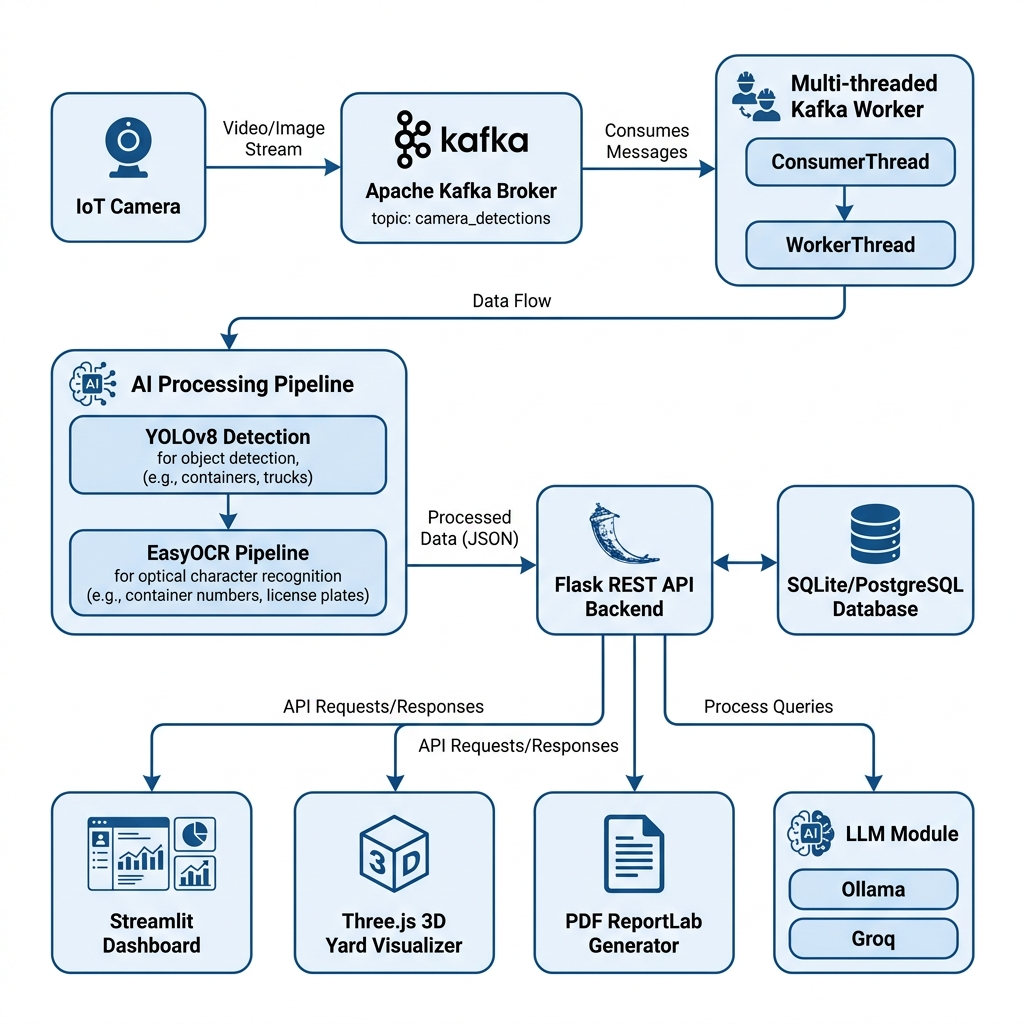
\includegraphics[width=\textwidth]{images/architecture_diagram.png}
    \caption{Représentation schématique de l'architecture YOLOv8 : extraction de caractéristiques multi-échelle et tête de prédiction découplée}
    \label{fig:yolov8_arch}
  \end{minipage}
\end{figure}

\subsubsection{Le Backbone (CSPDarknet53)}
Le Backbone fait office d'extracteur de caractéristiques principal. Il repose sur l'architecture CSPDarknet qui intègre des blocs C2f (variante optimisée du CSP block de YOLOv5). Ces blocs divisent les cartes de caractéristiques en deux canaux de traitement avant de les fusionner, ce qui permet d'enrichir la diversité des gradients tout en réduisant le coût de calcul.

\subsubsection{Le Neck (PANet)}
Le Neck sert à fusionner les caractéristiques extraites par le Backbone à différentes échelles géométriques. Il utilise un réseau d'agrégation de caractéristiques bidirectionnel FPN (Feature Pyramid Network) couplé à une structure PANet (Path Aggregation Network). Ce mécanisme permet de propager efficacement les informations sémantiques de haut niveau (formes globales) vers le bas, et les informations géométriques fines (contours, positions) vers le haut de la pyramide.

\subsubsection{Le Head (Decoupled Anchor-free Head)}
YOLOv8 introduit une rupture majeure au niveau de sa tête de détection :
\begin{itemize}
  \item \textbf{Decoupled Head (Tête Découplée)} : La classification (prédire la classe de l'objet) et la régression (prédire les coordonnées de la boîte) sont traitées par deux branches de convolutions distinctes, car ces deux tâches répondent à des caractéristiques différentes.
  \item \textbf{Anchor-Free (Sans Ancrage)} : Contrairement aux anciennes versions qui s'appuyaient sur des boîtes d'ancrage prédéfinies (\textit{anchor boxes}) ajustées manuellement par clustering K-Means, YOLOv8 prédit directement le centre de l'objet ainsi que la distance de ce centre aux quatre bords de l'objet. Cela réduit la complexité du réseau et le nombre d'hyperparamètres.
\end{itemize}

\subsubsection{Fonctions de Perte (Loss Functions) de YOLOv8}
L'apprentissage de la régression de boîte dans YOLOv8 repose sur deux pertes mathématiques avancées :
\begin{enumerate}
  \item \textbf{La perte CIoU (Complete Intersection over Union)} \cite{Zheng2020CIoU} : Elle pénalise l'écart entre la boîte prédite $B$ et la boîte réelle $B^{\text{gt}}$ en prenant en compte le chevauchement, la distance des centres et l'aspect ratio (proportions) :
  \begin{equation}
    \mathcal{L}_{\text{CIoU}} = 1 - \text{IoU} + \frac{\rho^2(b, b^{\text{gt}})}{c^2} + \alpha v
  \end{equation}
  Où $\text{IoU} = \frac{|B \cap B^{\text{gt}}|}{|B \cup B^{\text{gt}}|}$, $\rho(b, b^{\text{gt}})$ représente la distance euclidienne entre les centres des deux boîtes, $c$ est la longueur de la diagonale de la plus petite boîte englobant les deux boîtes, et :
  \begin{equation}
    v = \frac{4}{\pi^2} \left( \arctan \frac{w^{\text{gt}}}{h^{\text{gt}}} - \arctan \frac{w}{h} \right)^2, \quad \alpha = \frac{v}{(1 - \text{IoU}) + v}
  \end{equation}
  
  \item \textbf{La perte DFL (Distribution Focal Loss)} \cite{Li2020DFL} : Pour modéliser l'incertitude des frontières d'un objet (lorsque les contours sont flous dans l'image), YOLOv8 utilise la DFL. Au lieu de prédire une valeur unique de coordonnée, le réseau prédit une distribution de probabilité sur un intervalle discret $[y_i, y_{i+1}]$. La perte DFL force le réseau à concentrer les probabilités autour de la valeur réelle $y$ :
  \begin{equation}
    \mathcal{L}_{\text{DFL}}(y_i, y_{i+1}) = - \left( (y_{i+1} - y)\log(S_i) + (y - y_i)\log(S_{i+1}) \right)
  \end{equation}
  Où $S_i$ et $S_{i+1}$ sont les scores Softmax associés aux positions discrètes encadrant la valeur continue $y$.
\end{enumerate}

La perte globale d'apprentissage de YOLOv8 s'exprime donc par la combinaison linéaire :
\begin{equation}
  \mathcal{L} = \lambda_{\text{box}} \mathcal{L}_{\text{CIoU}} + \lambda_{\text{cls}} \mathcal{L}_{\text{BCE}} + \lambda_{\text{dfl}} \mathcal{L}_{\text{DFL}}
\end{equation}
Où $\mathcal{L}_{\text{BCE}}$ est la perte d'entropie croisée binaire pour la classification, et les coefficients $\lambda$ pondèrent les importances relatives des tâches.

\subsection{Reconnaissance Optique de Caractères (OCR) et Modèles Avancés}

L'OCR consiste à extraire la transcription textuelle de caractères imprimés sur une image. Les pipelines modernes d'OCR séparent cette tâche en deux étapes successives (voir figure~\ref{fig:ocr_pipeline_art}) : la détection de la boîte englobante du texte, puis la reconnaissance des caractères de cette zone.

\begin{figure}[H]
  \centering
  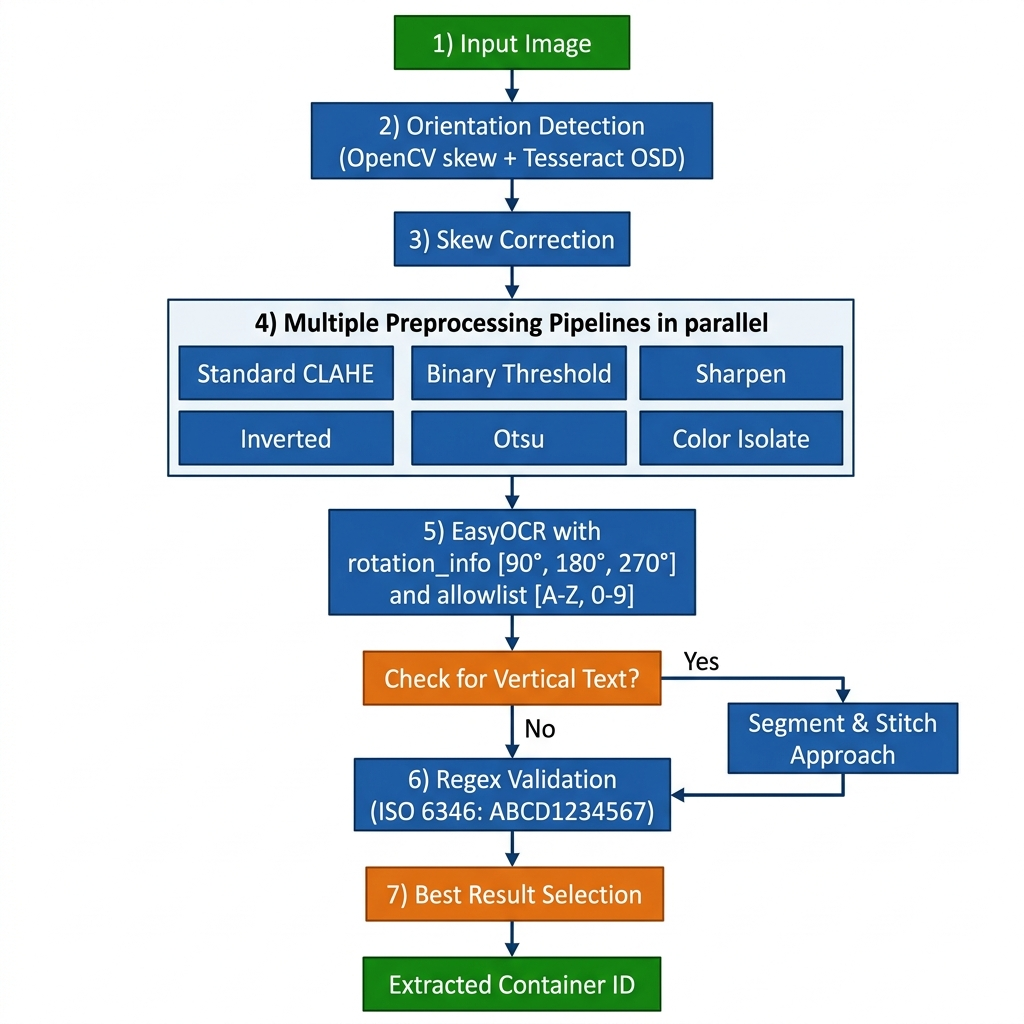
\includegraphics[width=0.90\textwidth]{images/ocr_pipeline_diagram.png}
  \caption{Architecture fonctionnelle d'un pipeline OCR divisé en détection de zone (CRAFT) et transcription de séquence (CRNN + CTC)}
  \label{fig:ocr_pipeline_art}
\end{figure}

Pour comprendre en profondeur le fonctionnement de notre pipeline, il est nécessaire de définir et d'expliquer trois concepts fondamentaux de l'état de l'art de l'OCR de Deep Learning : \ac{CRAFT}, \ac{CRNN} et la classification \ac{CTC}. Ces concepts décrivent la manière dont le système extrait les numéros d'immatriculation.

\subsubsection{Détection de texte : Modèle CRAFT}
Le modèle \textbf{CRAFT} (Character Region Awareness for Text Detection) \cite{Baek2019CRAFT} est conçu pour détecter du texte de forme arbitraire (courbe, orienté, incliné) dans des scènes réelles complexes. Contrairement aux anciens modèles de détection qui essayaient de deviner des blocs de mots entiers, CRAFT fonctionne au niveau du \textbf{caractère individuel}. 

Pour cela, CRAFT produit deux cartes d'activation pour chaque pixel de l'image :
\begin{itemize}
  \item \textbf{Region Score} (Score de Région) : Représente la probabilité qu'un pixel appartienne au centre d'un caractère individuel. Cela permet de repérer précisément chaque lettre ou chiffre, peu importe son orientation\,;
  \item \textbf{Affinity Score} (Score d'Affinité) : Représente la probabilité que deux caractères consécutifs soient liés pour former un mot ou une phrase. Cela permet de savoir si des lettres empilées ou côte à côte doivent être regroupées dans une même boîte de lecture.
\end{itemize}

\subsubsection{Reconnaissance de caractères : Réseau CRNN}
Une fois la boîte de texte détectée par CRAFT, elle est redressée (recadrée horizontalement) et envoyée à un réseau \textbf{CRNN} (Convolutional Recurrent Neural Network) \cite{Shi2016CRNN}. Ce modèle combine :
\begin{enumerate}
  \item \textbf{Des couches convolutives (CNN)} : Elles extraient une séquence de vecteurs de caractéristiques géométriques le long de la largeur de l'image du mot, en se focalisant sur les aspects visuels des formes de chaque lettre\,;
  \item \textbf{Des couches récurrentes (RNN / LSTM)} : Des couches récurrentes bidirectionnelles (Bidirectional LSTM) analysent l'ordre temporel des caractéristiques extraites. Cela permet de modéliser le contexte et les dépendances séquentielles\,;
  \item \textbf{Une couche de transcription} : Elle combine les sorties du LSTM pour restituer le code textuel final.
\end{enumerate}

\subsubsection{Transcription de séquence : La Perte CTC}
Le concept de \textbf{CTC} (Connectionist Temporal Classification) \cite{Graves2006CTC} est une technique mathématique essentielle pour entraîner des modèles de séquence (comme le texte ou la parole) sans avoir besoin d'aligner manuellement chaque caractère à sa position dans l'image.

En effet, lors du scan d'un mot, le réseau produit des prédictions pour chaque colonne verticale de pixels. Ainsi, pour l'image du mot "MSCU", le réseau pourrait prédire des doublons ou des vides : \texttt{M-S-S-C-U-U} (où \texttt{-} représente le caractère spécial "vide", noté $\epsilon$).
La couche CTC applique les règles de réduction suivantes :
\begin{itemize}
  \item Elle fusionne les caractères identiques consécutifs non séparés par un vide (ex. \texttt{S-S} devient \texttt{S})\,;
  \item Elle supprime tous les caractères vides $\epsilon$.
\end{itemize}
Ainsi, la séquence prédite \texttt{M-S-S-C-U-U} est instantanément simplifiée en \texttt{MSCU}.

\subsection{Apache Kafka -- Streaming de Données Temps Réel}

Pour concevoir un système industriel capable de traiter les images de caméras à haute fréquence sans congestionner le serveur de base de données ni bloquer l'interface graphique, l'utilisation d'une architecture de messagerie distribuée est indispensable \cite{Kafka}.

Apache Kafka est une plateforme de diffusion d'événements distribuée, hautement tolérante aux pannes et conçue pour ingérer des flux de données en continu. Son fonctionnement repose sur le modèle de publication-souscription (\textit{Publish-Subscribe}) :
\begin{itemize}
  \item \textbf{Topics} : Les flux de données sont organisés et stockés dans des catégories appelées topics (\texttt{camera\_detections}, \texttt{container\_ids}).
  \item \textbf{Partitions} : Chaque topic est divisé en plusieurs partitions réparties sur les serveurs du cluster (Brokers).
  \item \textbf{Producers / Consumers} : Les producteurs publient les messages et les consommateurs (regroupés en \textbf{Consumer Groups}) les traitent en parallèle.
  \item \textbf{Offsets} : Identifiants de position permettant un redémarrage sans perte de données.
\end{itemize}

\subsection{Le Problème de l'Allocation de Parc (Yard Stacking Problem)}

La logistique portuaire s'intéresse de près au positionnement optimal des conteneurs pour minimiser les doubles manipulations. En recherche opérationnelle, ce problème est désigné sous le nom de \textit{Container Relocation Problem} (CRP) ou \textit{Yard Stacking Problem} (YSP). Il a été formellement prouvé comme étant \textbf{NP-difficile} au sens fort par réduction du problème de coloration de graphes orientés et du problème du sac à dos \cite{Caserta2011, Kim2002, Jin2015}.

\subsubsection{Formulation mathématique}
Soit un parc de stockage composé d'un ensemble de piles $S$. Chaque pile $s \in S$ possède une capacité maximale en hauteur notée $H_s$.
Chaque conteneur physique $c$ arrivant au port possède des attributs connus : sa taille $L(c) \in \{20, 40\}$ pieds, son poids $W(c) \in \mathbb{R}^+$, et sa date de départ prévue $D(c) \in \mathbb{R}^+$.

Lorsqu'un nouveau conteneur $c_{\text{new}}$ doit être placé sur une pile $s$, il est empilé au-dessus du conteneur supérieur actuel $c_{\text{top}}$.
Pour éviter toute double manipulation future, la règle de priorité d'échéance (\ac{EDD}) doit être satisfaite \cite{Baker2009} :
\begin{equation}
  D(c_{\text{new}}) \geq D(c_{\text{top}})
\end{equation}
De plus, la contrainte de stabilité physique de poids impose que :
\begin{equation}
  W(c_{\text{new}}) \le W(c_{\text{top}})
\end{equation}

\subsubsection{Algorithme du Recuit Simulé et Formalisation de la Fonction de Coût}
Lorsque le parc est très encombré (taux d'occupation $> 70\,\%$), il devient impossible de respecter strictement toutes ces contraintes sur toutes les piles. Nous utilisons la métaheuristique du \textbf{Recuit Simulé} (\ac{SA}) \cite{Kirkpatrick1983} pour explorer l'espace des solutions sans bloquer dans des minima locaux.

Nous formalisons explicitement la fonction de coût (énergie $E(s)$) minimisée par l'algorithme pour évaluer un placement candidat du conteneur $c_{\text{new}}$ sur une pile $s$ :
\begin{equation}
  E(s) = w_1 \cdot \mathbb{I}\left(D(c_{\text{new}}) < D(c_{\text{top}})\right) + w_2 \cdot \mathbb{I}\left(W(c_{\text{new}}) > W(c_{\text{top}})\right) + w_3 \cdot \frac{D_{\text{quai}}(s)}{D_{\max}} + w_4 \cdot \frac{H_s}{H_{\max}}
\end{equation}
Où $\mathbb{I}(\cdot)$ est l'indicateur de violation de contrainte, $D_{\text{quai}}(s)$ est la distance manhattanienne entre le quai STS et la pile $s$, et $H_s/H_{\max}$ pénalise la saturation en hauteur. Les poids retenus après réglage empirique sont $w_1 = 50.0$ (pénalité majeure de EDD), $w_2 = 30.0$ (pénalité de poids), $w_3 = 10.0$ et $w_4 = 10.0$.

L'algorithme de Boltzmann gouverne l'acceptation des dégradations d'énergie à température $T$ :
\begin{equation}
  P(\text{acceptation}) = \exp\left(-\frac{\Delta E}{T}\right)
\end{equation}
Le schéma de refroidissement géométrique s'exécute selon $T_{k+1} = \alpha \cdot T_k$. Les hyperparamètres retenus pour le déploiement sont : température initiale $T_0 = 100.0$, facteur de refroidissement $\alpha = 0.90$, température minimale $T_{\min} = 0.1$, et $N_{\text{iter}} = 10$ explorations locales par palier de température.

\subsection{Travaux Connexes et Positionnement Scientifique}

Afin de situer notre contribution par rapport à l'état de l'art international, nous avons mené une étude comparative des travaux scientifiques récents portant sur l'identification automatique de conteneurs et l'optimisation du stockage portuaire. Le tableau~\ref{tab:related_work} résume ce positionnement.

\begin{table}[H]
\centering
\caption{Tableau comparatif des travaux connexes récents et positionnement de notre étude}
\begin{tabular}{|p{3cm}|c|p{3.5cm}|p{3.5cm}|p{3cm}|}
\hline
\rowcolor{TableHeader}\textcolor{white}{\textbf{Auteurs \& Année}} & \textcolor{white}{\textbf{Domaine}} & \textcolor{white}{\textbf{Méthode proposée}} & \textcolor{white}{\textbf{Performances / Résultats}} & \textcolor{white}{\textbf{Limites vs Notre Approche}} \\ \hline
Kim et al. (2020) \cite{Kim2020ISO} & OCR ISO & YOLOv3 + Tesseract & Taux de lecture 76,2\,\% sur texte horizontal & Échec sur codes verticaux, pas d'optimisation parc \\ \hline
Jin et al. (2021) \cite{Jin2021CRP} & Stacking & Program. Dynamique / Heuristique & Réduction re-handling 45\,\% & Temps de calcul élevé ($> 30$\,s), pas de vision \\ \hline
Zhang \& Lin (2022) \cite{Zhang2022OCR} & OCR Code & CRAFT + CRNN personnalisée & Taux de lecture 91,0\,\% (dataset propre) & Nécessite GPU dédié, pas d'ingestion streaming Kafka \\ \hline
Caserta et al. (2023) \cite{Caserta2023YSP} & Stacking & Métaheuristique GRASP + ILS & Optimisation offline du yard & Traitement par batch non adapté au temps réel quai \\ \hline
\textbf{Notre Solution (2026)} & \textbf{Vision + Yard} & \textbf{YOLOv8 + Segment-Stitch + Kafka + EDD-SA} & \textbf{OCR 85,0\,\% (h+v), Re-handling $< 12\,\%$, Latence 1,3\,s} & \textbf{Plateforme industrielle complète de bout en bout} \\ \hline
\end{tabular}
\label{tab:related_work}
\end{table}

\subsection{Bilan du Chapitre 2}
En conclusion, ce deuxième chapitre a exposé les fondements théoriques des trois piliers technologiques du projet : la détection visuelle par YOLOv8, la lecture optique robuste (CRAFT, CRNN, CTC), le streaming distribué temps réel (Kafka) et la modélisation de l'allocation du parc par Recuit Simulé. Nous avons formalisé la fonction de coût $E(s)$, justifié la complexité NP-difficile du problème et positionné notre travail face aux publications récentes. Le chapitre suivant présente la conception générale et l'architecture logicielle du système.

\newpage

% ═══════════════════════════════════════════════════════════════════
% CHAPITRE 3 — CONCEPTION GÉNÉRALE ET ARCHITECTURE
% ═══════════════════════════════════════════════════════════════════
\section{Conception Générale et Architecture du Système}

Ce chapitre présente la structure globale de la plateforme, les flux d'informations transitant entre les composants de l'infrastructure portuaire, la modélisation logique de la base de données relationnelle ainsi que la spécification des interfaces de programmation (endpoints REST).

\subsection{Architecture Globale et Flux de Données}

Pour garantir la résilience, la modularité et l'extensibilité du système, nous avons opté pour une \textbf{architecture orientée microservices}. La figure~\ref{fig:architecture_conceptuelle} présente le diagramme conceptuel d'architecture physique et logique de notre solution.

\begin{figure}[H]
  \centering
  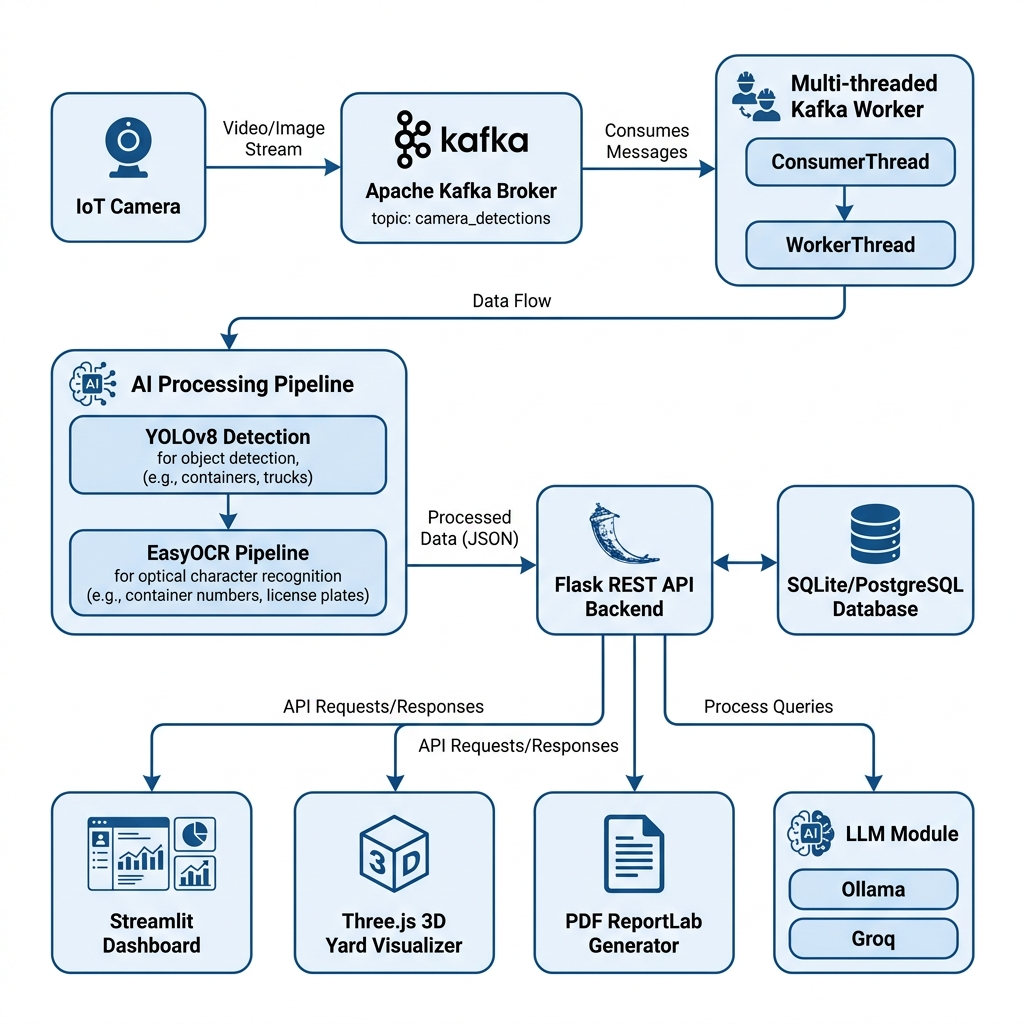
\includegraphics[width=0.95\textwidth]{images/architecture_diagram.png}
  \caption{Architecture globale de la solution Port Logistics AI avec intégration IoT et streaming asynchrone}
  \label{fig:architecture_conceptuelle}
\end{figure}

Le fonctionnement de l'architecture suit un flux d'événements rigoureux :
\begin{enumerate}
  \item \textbf{Ingestion} : Le script caméra IoT (\texttt{realtime\_camera.py}) simule une caméra IP montée sur le portique de quai. Il capture le flux vidéo et utilise une boucle de détection locale ultra-légère YOLOv8. Si la présence d'un conteneur est détectée de manière stable pendant 2 secondes, la frame correspondante est convertie en Base64.
  \item \textbf{Messagerie} : La frame, enrichie de métadonnées opérationnelles (navire, quai, opérateur), est enveloppée dans un message JSON et publiée dans le topic Kafka \texttt{camera\_detections}.
  \item \textbf{Traitement Asynchrone} : Le worker d'arrière-plan (\texttt{kafka\_worker.py}) consomme les messages du topic Kafka. Pour chaque message, il décode l'image et l'envoie au pipeline de Vision par Ordinateur. YOLOv8n localise les conteneurs et extrait les coordonnées géométriques, puis le module OCR analyse les crops d'image pour transcrire les caractères ISO 6346.
  \item \textbf{Persistance \& Logique métier} : Le worker communique avec l'API Flask backend pour sauvegarder l'historique et interroger le manifeste navire. Si le code conteneur extrait correspond à une entrée du manifeste, l'API interroge le service d'optimisation (\texttt{yard\_optimizer.py}) pour calculer l'emplacement physique optimal dans le parc.
  \item \textbf{Supervision} : L'interface utilisateur Streamlit communique avec l'API REST de Flask pour afficher en temps réel les indicateurs de performance logistique, l'état physique du yard sous forme de rendu 3D interactif (Three.js WebGL canvas) et déclencher la génération de rapports PDF enrichis par LLM.
\end{enumerate}

\subsection{Conception Globale : Diagramme de Packages}

Afin de garantir la modularité et la séparation des responsabilités, le code source a été structuré en packages logiques cohérents. La Figure~\ref{fig:packages_diagram} présente le diagramme de packages logiques de l'application.

\begin{figure}[H]
  \centering
  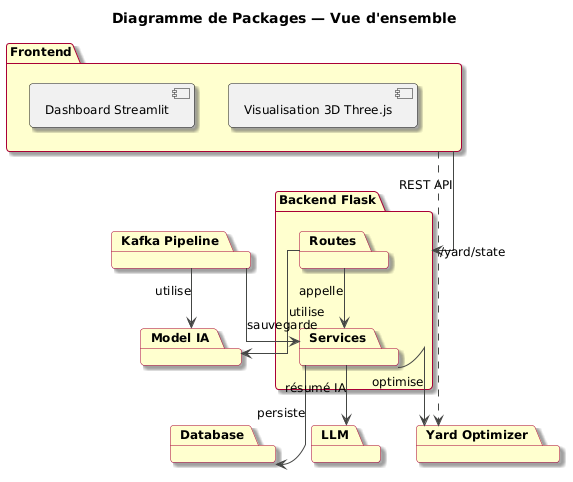
\includegraphics[width=0.90\textwidth]{diagrames/Diagram_packege.png}
  \caption{Découpage en packages logiques de l'application}
  \label{fig:packages_diagram}
\end{figure}

\subsection{Modélisation Fonctionnelle : Diagramme de Cas d'Utilisation}

Le diagramme de cas d'utilisation (Figure~\ref{fig:use_case}) décrit de manière fonctionnelle les interactions entre les différents acteurs (l'opérateur STS, l'administrateur, le système de messagerie de la caméra et le service LLM) et les fonctionnalités majeures fournies par notre système.

\begin{figure}[H]
  \centering
  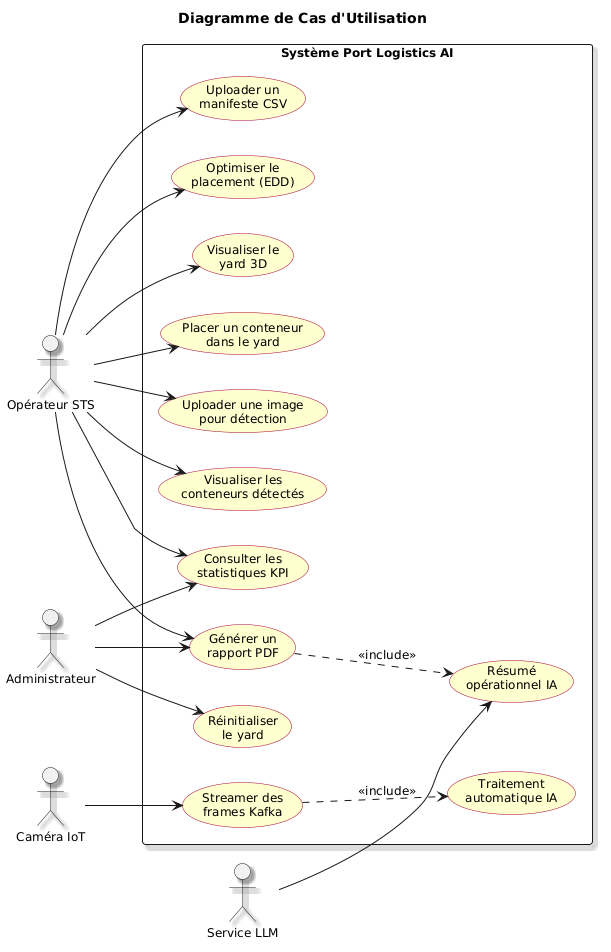
\includegraphics[width=0.90\textwidth]{diagrames/diagrame-use_case.png}
  \caption{Diagramme de cas d'utilisation du système}
  \label{fig:use_case}
\end{figure}

\subsection{Modélisation de la Base de Données}

La structure logique de la base de données relationnelle a été conçue pour refléter fidèlement l'état physique du terminal tout en optimisant les temps de requête pour l'affichage en temps réel. La Figure~\ref{fig:er_schema} présente le schéma conceptuel et relationnel de notre base de données.

\begin{figure}[H]
  \centering
  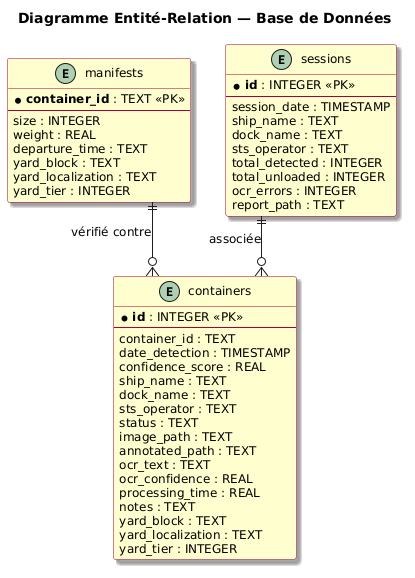
\includegraphics[width=0.85\textwidth]{diagrames/diagrame_entite_relation.png}
  \caption{Schéma relationnel logique de la base de données portuaire}
  \label{fig:er_schema}
\end{figure}

Le schéma comporte trois tables principales :

\subsubsection{La table \texttt{containers}}
C'est la table centrale du système qui enregistre chaque événement physique de détection survenu sous un portique. Elle mémorise l'historique complet des passages, la confiance des modèles de deep learning et les coordonnées finales d'affectation spatiale calculées par l'optimiseur. Elle est modélisée par la classe ORM SQLAlchemy \texttt{Container}.

\subsubsection{La table \texttt{manifests}}
Elle contient les informations prévisionnelles de chargement des navires importées par les compagnies maritimes. Le manifeste sert de table de référence pour valider l'intégrité de la lecture OCR et récupérer des données essentielles à l'optimisation comme le poids réel et la date d'échéance de sortie prévue. Elle est représentée par la classe ORM \texttt{ManifestContainer}.

\subsubsection{La table \texttt{sessions}}
Elle sert à enregistrer le bilan d'activité des équipes portuaires par cycle de travail (quart/shift). Elle garde une trace aggregée des déchargements d'un navire à un quai donné pour faciliter la génération automatique de rapports par le LLM. Elle est matérialisée par la classe ORM \texttt{DetectionSession}.

\subsection{Spécification de l'API REST Backend}

Le backend Flask expose ses services métier sous forme d'API REST structurée en blueprints modulaires. Le tableau~\ref{tab:api_endpoints} détaille la spécification des interfaces de programmation.

\begin{table}[H]
\centering
\caption{Spécifications exhaustives de l'API Flask REST}
\begin{tabular}{|l|p{4cm}|p{7.5cm}|}
\hline
\rowcolor{TableHeader}\textcolor{white}{\textbf{Méthode}} & \textcolor{white}{\textbf{Endpoint}} & \textcolor{white}{\textbf{Description / Rôle}} \\ \hline
\texttt{GET} & \texttt{/health} & Vérification de l'état des services et de la connexion BD.\\ \hline
\texttt{POST} & \texttt{/detect} & Réception d'image brute par formulaire HTTP, exécution YOLOv8 + OCR en mode synchrone (fallback).\\ \hline
\texttt{GET} & \texttt{/containers} & Récupération de la liste paginée des conteneurs détectés avec filtres de statut.\\ \hline
\texttt{GET} & \texttt{/stats} & Agrégation des KPIs clés (taux d'erreur OCR, moyennes de confiance, volumes quotidiens).\\ \hline
\texttt{GET} & \texttt{/reports/generate} & Déclenchement de la compilation du rapport PDF hebdomadaire (ReportLab + synthèse LLM).\\ \hline
\texttt{GET} & \texttt{/yard/state} & Extraction de la configuration tridimensionnelle du parc de stockage (format JSON structuré pour Three.js).\\ \hline
\texttt{POST} & \texttt{/yard/optimize} & Exécution de l'algorithme d'optimisation (EDD + Recuit Simulé) pour un conteneur donné.\\ \hline
\texttt{POST} & \texttt{/yard/place} & Confirmation et validation physique du placement d'un conteneur à des coordonnées géographiques précises.\\ \hline
\texttt{DELETE} & \texttt{/yard/reset} & Réinitialisation complète du parc (suppression physique de tous les conteneurs stockés).\\ \hline
\texttt{POST} & \texttt{/manifest/upload} & Importation en base de données d'un fichier CSV représentant le manifeste théorique d'un navire.\\ \hline
\end{tabular}
\label{tab:api_endpoints}
\end{table}

\subsection{Conception Statique : Diagrammes de Classes}

Pour surmonter les limites de lisibilité sur des pages de rapport au format A4, le diagramme de classes général a été scindé en plusieurs diagrammes thématiques représentant chacun un module autonome du système.

\subsubsection{Module Base de Données et Entités ORM}
Le diagramme de la Figure~\ref{fig:class_db} détaille la structure des tables SQL représentées par des classes ORM SQLAlchemy, ainsi que l'interface \texttt{DBManager} qui encapsule les opérations de persistance (CRUD).

\begin{figure}[H]
  \centering
  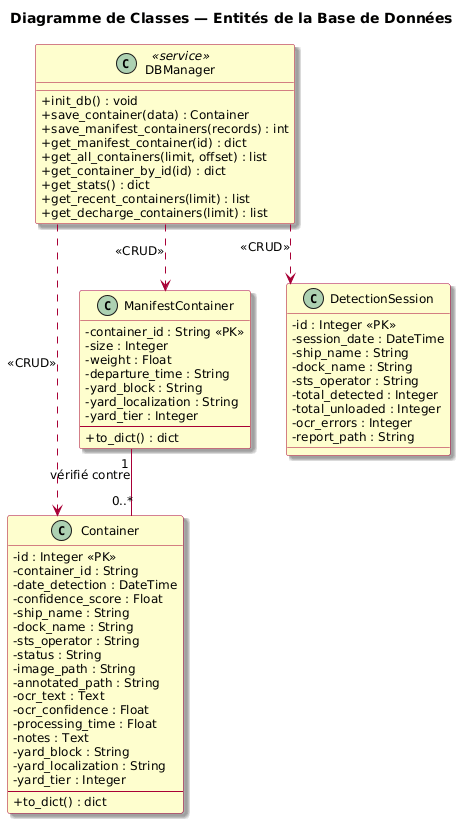
\includegraphics[width=0.90\textwidth]{diagrames/diagrame_classe.png}
  \caption{Diagramme de classes du module Base de données et Persistance}
  \label{fig:class_db}
\end{figure}

\subsubsection{Module Intelligence Artificielle (YOLOv8 \& EasyOCR)}
La Figure~\ref{fig:class_ia} présente les classes du module de traitement d'image et d'OCR. La classe \texttt{ContainerDetector} localise les conteneurs et fournit des crops d'image à la classe \texttt{OCRReader} pour en extraire le code ISO 6346.

\begin{figure}[H]
  \centering
  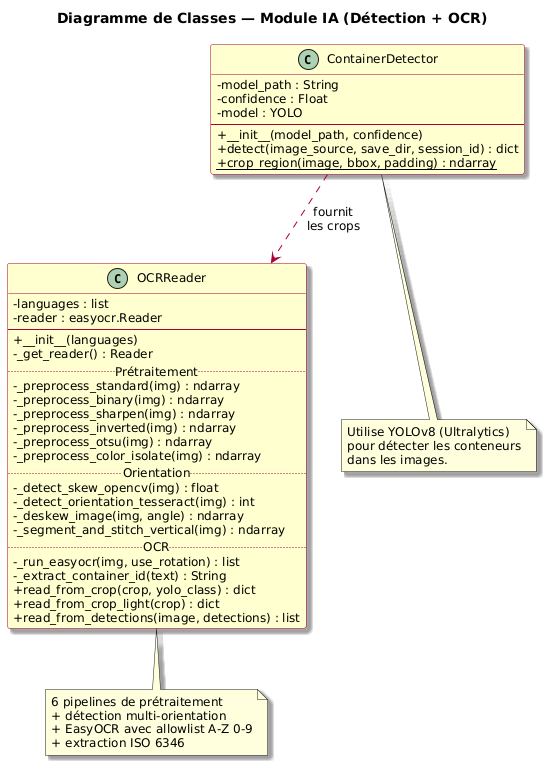
\includegraphics[width=0.90\textwidth]{diagrames/diagram_classe_Module_IA_Detection_OCR.png}
  \caption{Diagramme de classes du module de Vision par Ordinateur et OCR}
  \label{fig:class_ia}
\end{figure}

\subsubsection{Module Yard Optimizer}
La Figure~\ref{fig:class_yard} montre les structures logiques modélisant le parc physique (Yard, Block, Stack, Slot) et la logique d'ordonnancement mise en œuvre par l'algorithme d'optimisation.

\begin{figure}[H]
  \centering
  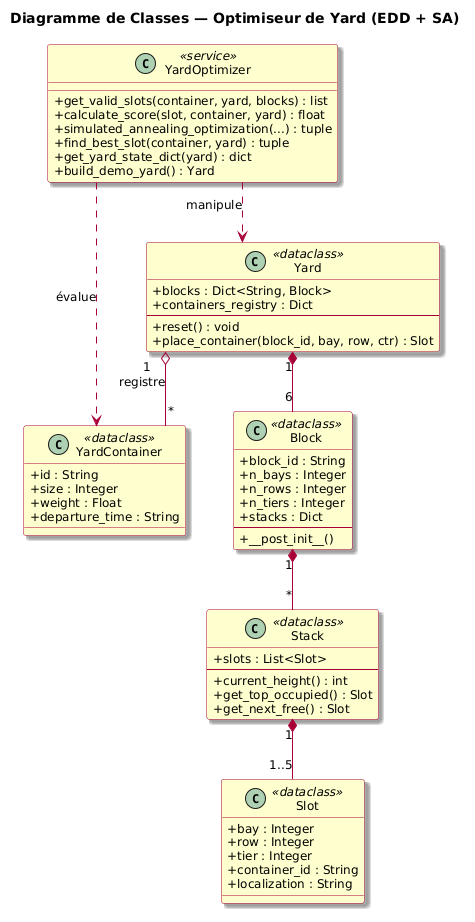
\includegraphics[width=0.90\textwidth]{diagrames/diagrame_classe_Yard_Optimizer.png}
  \caption{Diagramme de classes de l'optimiseur de placement dans le parc}
  \label{fig:class_yard}
\end{figure}

\subsubsection{Module de Reporting et Assistant LLM}
Le diagramme de la Figure~\ref{fig:class_report} montre les relations entre le générateur de rapport PDF et le module d'intelligence artificielle chargé de rédiger des résumés textuels.

\begin{figure}[H]
  \centering
  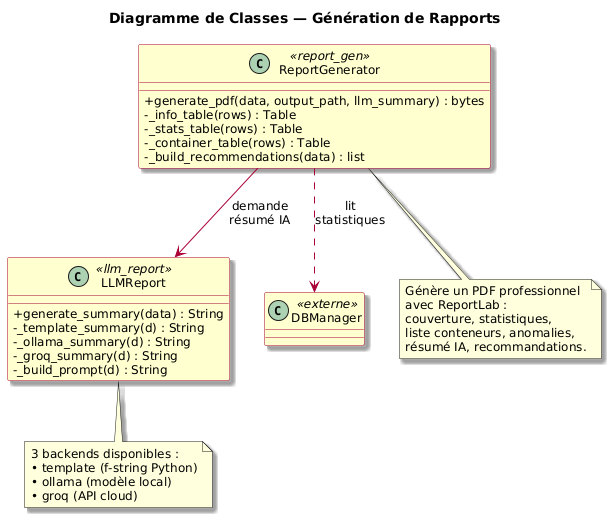
\includegraphics[width=0.90\textwidth]{diagrames/diagrame_classe_repport_llm.png}
  \caption{Diagramme de classes du module de reporting et d'intégration LLM}
  \label{fig:class_report}
\end{figure}

\subsection{Conception Dynamique : Diagrammes de Séquence}

Les scénarios d'utilisation principaux du système impliquent des interactions temporelles entre les composants du backend, de l'IA, de la base de données et du streaming.

\subsubsection{Scénario d'Identification de Conteneur via Upload HTTP}
La Figure~\ref{fig:seq_upload} détaille le flux synchrone déclenché lorsqu'un opérateur importe une image de conteneur depuis le dashboard pour l'identifier et vérifier son statut avec le manifeste.

\begin{figure}[H]
  \centering
  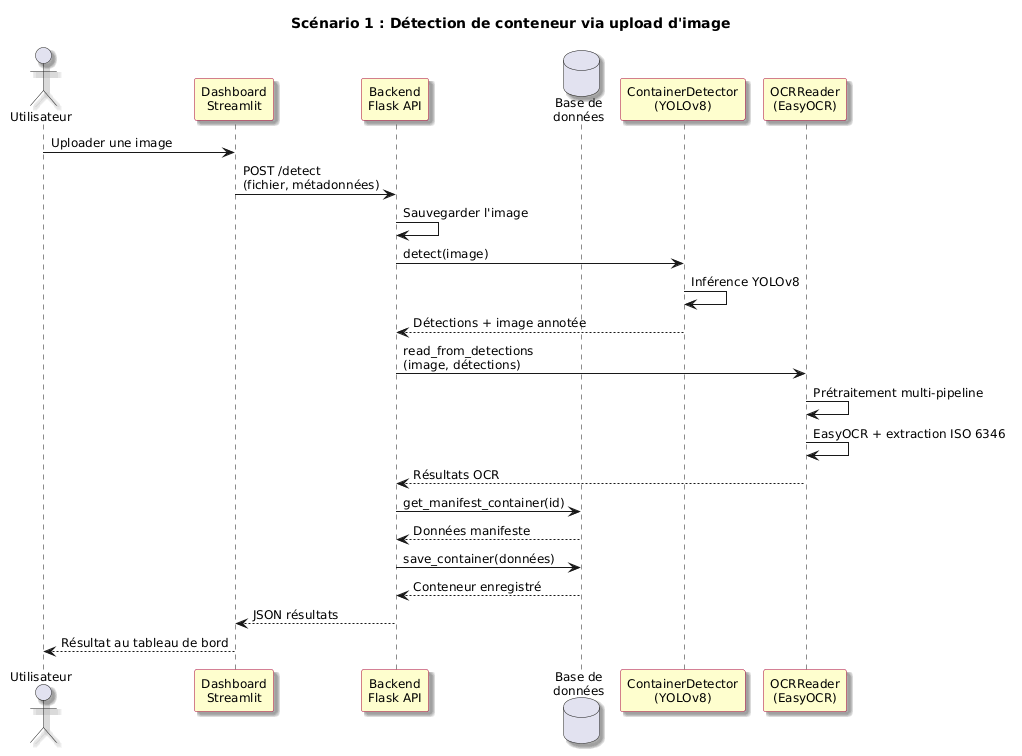
\includegraphics[width=0.90\textwidth]{diagrames/sequence_detection_upload.png}
  \caption{Diagramme de séquence pour le traitement synchrone via upload d'image}
  \label{fig:seq_upload}
\end{figure}

\subsubsection{Scénario d'Optimisation du Placement dans le Yard}
La Figure~\ref{fig:seq_yard} montre les étapes de calcul et d'affectation spatiale d'un conteneur dans le parc logistique à l'aide de l'algorithme EDD et du Recuit Simulé.

\begin{figure}[H]
  \centering
  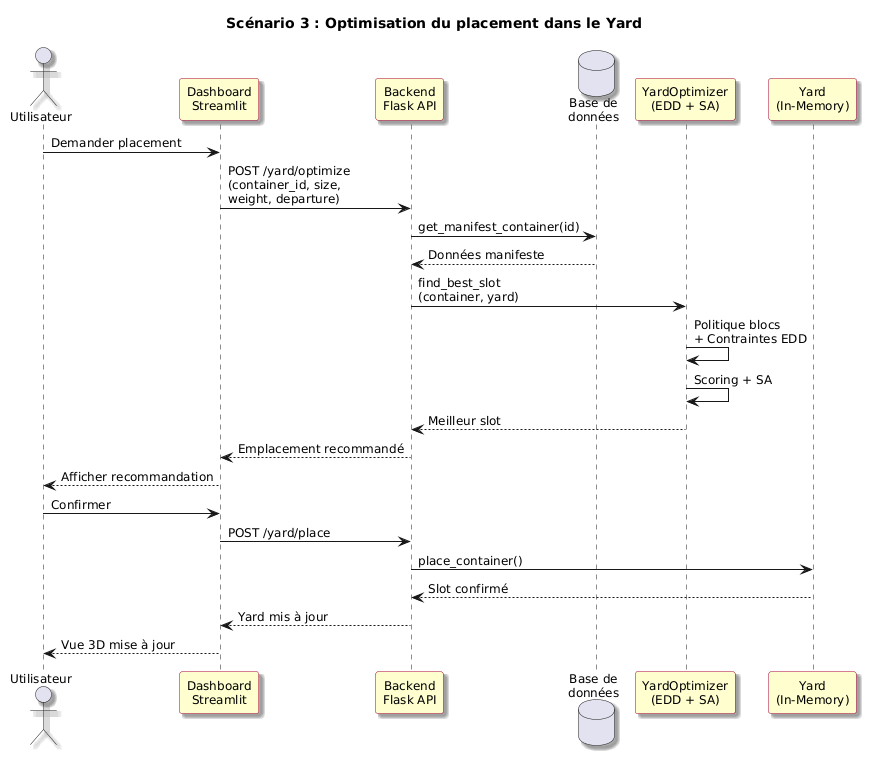
\includegraphics[width=0.90\textwidth]{diagrames/sequence_yard_optimisation.png}
  \caption{Diagramme de séquence pour l'optimisation du placement}
  \label{fig:seq_yard}
\end{figure}

\subsection{Conception des Processus : Diagrammes d'Activité et d'État}

Les logiques algorithmiques et logistiques internes de traitement sont modélisées par des diagrammes d'activité et d'état.

\subsubsection{Diagramme d'Activité : Pipeline OCR Multi-Orientation}
La Figure~\ref{fig:act_ocr} présente l'algorithme de lecture robuste, détaillant les rotations de recalage géométrique, le traitement des codes verticaux (Segment-and-Stitch), l'application séquentielle des 6 pipelines de prétraitement et le critère d'arrêt anticipé.

\begin{figure}[H]
  \centering
  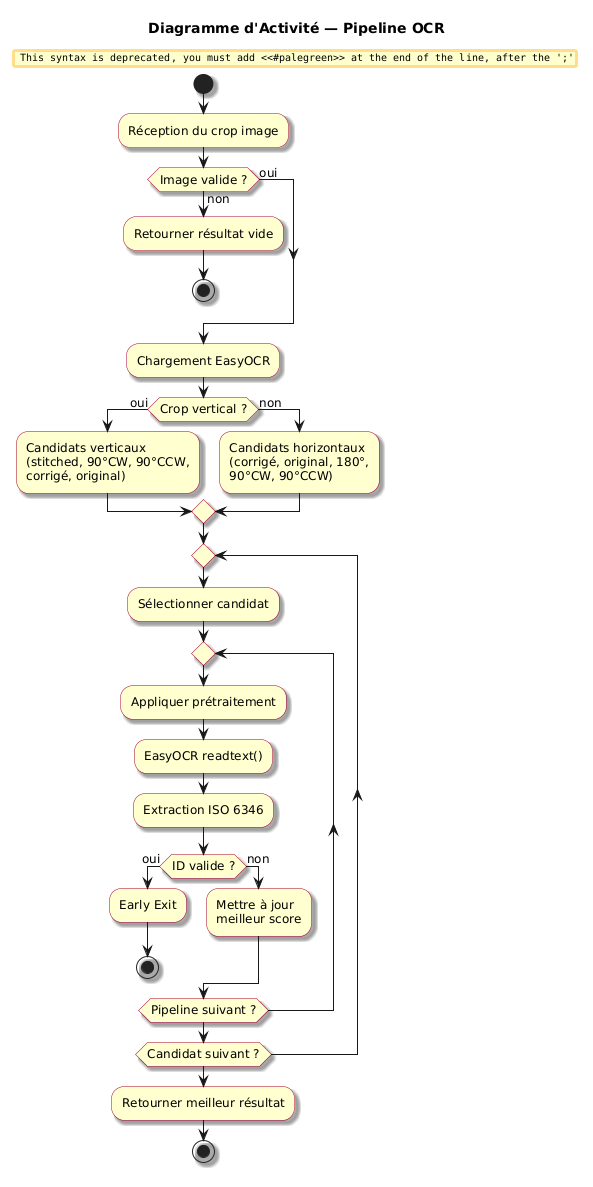
\includegraphics[width=0.90\textwidth]{diagrames/actevie_ocr_pipline.png}
  \caption{Diagramme d'activité de l'OCR multi-orientation}
  \label{fig:act_ocr}
\end{figure}

\subsubsection{Diagramme d'État : Cycle de vie d'un Conteneur}
La Figure~\ref{fig:state_ctr} modélise les différents états logiques par lesquels passe un conteneur au sein du terminal portuaire, depuis sa détection quai jusqu'à son chargement à bord d'un navire.

\begin{figure}[H]
  \centering
  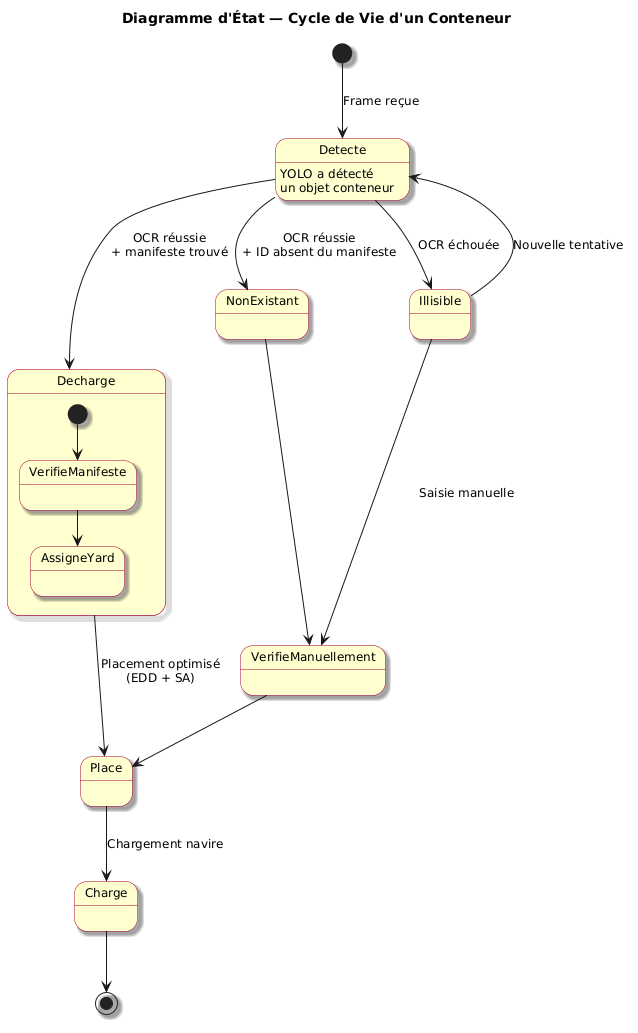
\includegraphics[width=0.90\textwidth]{diagrames/diagrame_etat_cycle_vie_contenure.png}
  \caption{Diagramme d'état pour le cycle de vie d'un conteneur}
  \label{fig:state_ctr}
\end{figure}

\subsection{Architecture de Déploiement Conteneurisée}

Afin de simplifier le déploiement sur les serveurs de production de Marsa Maroc, toute l'infrastructure a été conteneurisée à l'aide de Docker. Un fichier d'orchestration centralisé \texttt{docker-compose.yml} coordonne l'exécution et l'interconnexion de cinq conteneurs isolés :
\begin{enumerate}
  \item \textbf{Le conteneur Base de Données (PostgreSQL)} : Assure le stockage des données opérationnelles de manière persistante sur un volume Docker dédié.
  \item \textbf{Le conteneur de Messagerie (Kafka \& Zookeeper)} : Gère les topics et assure le transit des messages temps réel entre le quai et les instances IA.
  \item \textbf{Le conteneur Backend (API Flask)} : Expose l'API de logique métier sur le réseau.
  \item \textbf{Le conteneur Worker IA (Kafka Worker)} : Contient les dépendances de deep learning (PyTorch, Ultralytics, EasyOCR). Il partage les modèles et exécute en continu l'inférence.
  \item \textbf{Le conteneur Frontend (Streamlit Dashboard)} : Présente l'interface web accessible par le réseau local de l'entreprise.
\end{enumerate}

La Figure~\ref{fig:deployment} présente la cartographie de déploiement réseau et matériel de cette infrastructure conteneurisée.

\begin{figure}[H]
  \centering
  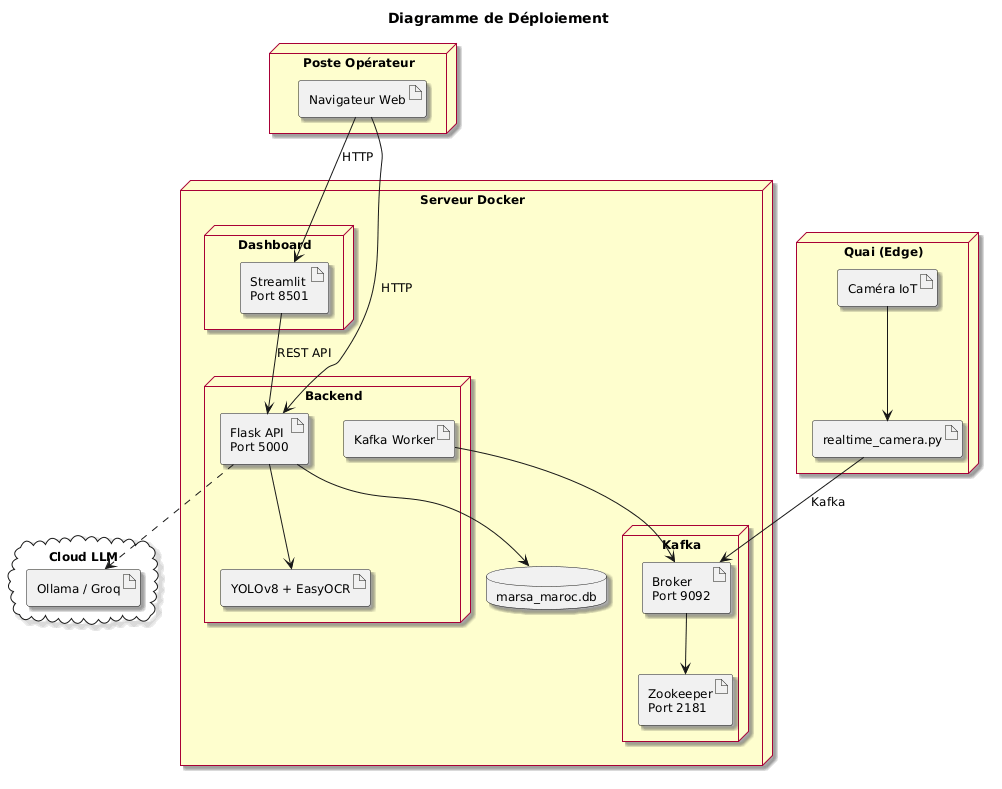
\includegraphics[width=0.90\textwidth]{diagrames/diagrame_deploiement.png}
  \caption{Diagramme de déploiement physique du système Port Logistics AI}
  \label{fig:deployment}
\end{figure}

\subsection{Bilan du Chapitre 3}
Ce troisième chapitre a détaillé la conception logicielle et l'architecture système de notre plateforme. Nous avons modélisé les microservices, la base de données relationnelle, l'API REST, les diagrammes UML (classes, séquence, activité, état) et le déploiement conteneurisé sous Docker. Le chapitre suivant aborde l'implémentation technique des composants et la présentation des interfaces applicatives.

\newpage

% ═══════════════════════════════════════════════════════════════════
% CHAPITRE 4 — IMPLÉMENTATION ET DÉVELOPPEMENT
% ═══════════════════════════════════════════════════════════════════
\section{Implémentation et Développement de la Solution}

Ce chapitre présente les choix d'implémentation logicielle des briques applicatives principales. Afin d'assurer une lisibilité optimale, les extraits de code présentés dans ce chapitre sont restreints aux 15 à 20 lignes clés réellement discutées, tandis que les listings complets sont regroupés dans l'Annexe~A. Ce chapitre s'achève par la démonstration fonctionnelle illustrée des interfaces de la plateforme.

\subsection{Modélisation SQLAlchemy ORM}

Les modèles relationnels sont déclarés dans le fichier \texttt{backend/services/db\_manager.py}. L'extrait ci-dessous présente la structure des entités ORM principales \texttt{Container} et \texttt{ManifestContainer} :

\begin{vscodeWindow}{db\_manager.py}
class Container(Base):
    __tablename__ = "containers"

    id               = Column(Integer, primary_key=True, autoincrement=True)
    container_id     = Column(String(50))
    date_detection   = Column(DateTime, default=datetime.utcnow)
    confidence_score = Column(Float)
    status           = Column(String(50), default="detecte")
    ocr_text         = Column(Text)
    ocr_confidence   = Column(Float)
    processing_time  = Column(Float)
    
    # Coordonnees spatiales d'affectation dans le Yard
    yard_block        = Column(String(10), nullable=True)
    yard_localization = Column(String(50), nullable=True)
    yard_tier         = Column(Integer, nullable=True)
\end{vscodeWindow}

\subsection{Module de Vision par Ordinateur -- YOLOv8 Wrapper}

La détection des conteneurs sur les flux vidéo de surveillance quai est gérée par le composant \texttt{ContainerDetector} situé dans \texttt{model/container\_detector.py}. Il encapsule le modèle YOLOv8n pour réaliser l'inférence et découper les zones d'intérêt :

\begin{vscodeWindow}{container\_detector.py}
class ContainerDetector:
    def __init__(self, model_path: str = "yolov8n.pt", confidence: float = 0.40):
        self.model = YOLO(model_path)
        self.confidence = confidence

    def detect(self, image_source: str | np.ndarray) -> dict:
        results = self.model.predict(source=image_source, conf=self.confidence, verbose=False)
        detections = []
        if results and len(results) > 0:
            for box in results[0].boxes:
                x1, y1, x2, y2 = map(int, box.xyxy[0].tolist())
                detections.append({
                    "bbox": [x1, y1, x2, y2],
                    "confidence": round(float(box.conf[0]), 4)
                })
        return {"detections": detections}
\end{vscodeWindow}

\subsection{Pipeline OCR Robuste et Algorithme Segment-and-Stitch}

Le composant \texttt{backend/services/ocr\_reader.py} implémente l'extraction textuelle des codes ISO 6346. Il intègre la méthode \texttt{\_segment\_and\_stitch\_vertical} qui isole les caractères verticaux et les réassemble horizontalement :

\begin{vscodeWindow}{ocr\_reader.py}
@staticmethod
def _segment_and_stitch_vertical(img: np.ndarray) -> np.ndarray | None:
    h, w = img.shape[:2]
    if h <= w * 1.2:
        return None # Image non verticale
        
    gray = cv2.cvtColor(img, cv2.COLOR_BGR2GRAY)
    _, thresh = cv2.threshold(gray, 0, 255, cv2.THRESH_BINARY + cv2.THRESH_OTSU)
    num_labels, labels, stats, centroids = cv2.connectedComponentsWithStats(thresh)
    
    # Selection et tri vertical des composantes connexes
    components = sorted([{"bbox": (stats[i][0], stats[i][1], stats[i][2], stats[i][3]), "y": stats[i][1]} 
                        for i in range(1, num_labels) if stats[i][4] >= 25], key=lambda c: c["y"])
    
    # Redimensionnement et assemblage horizontal
    crops = [cv2.resize(img[c["y"]:c["y"]+c["bbox"][3], c["bbox"][0]:c["bbox"][0]+c["bbox"][2]], (30, 100)) for c in components]
    return np.hstack(crops) if len(crops) >= 4 else None
\end{vscodeWindow}

\subsection{Moteur d'Optimisation du Stacking du Parc (Yard Optimizer)}

Le fichier \texttt{backend/services/yard\_optimizer.py} contient l’implémentation de la métaheuristique du Recuit Simulé et le filtrage des emplacements valides selon la règle EDD :

\begin{vscodeWindow}{yard\_optimizer.py}
def simulated_annealing_optimization(container: Container, yard: Yard, valid_slots: List[Tuple[str, Slot]], 
                                     initial_temp: float = 100.0, cooling_rate: float = 0.90) -> Tuple[Tuple[str, Slot], float]:
    current = random.choice(valid_slots)
    current_cost = calculate_score(current[1], container, yard)
    best, best_cost = current, current_cost
    T = initial_temp
    
    while T > 0.1:
        neighbour = random.choice(valid_slots)
        n_cost = calculate_score(neighbour[1], container, yard)
        delta = n_cost - current_cost
        if delta < 0 or random.random() < math.exp(-delta / T):
            current, current_cost = neighbour, n_cost
            if current_cost < best_cost:
                best, best_cost = current, current_cost
        T *= cooling_rate
    return best, best_cost
\end{vscodeWindow}

\subsection{Worker Asynchrone Multi-Threadé}

Pour lier Kafka et l'inférence IA sans bloquer la réception des images, le worker \texttt{backend/services/kafka\_worker.py} s'appuie sur deux threads synchronisés avec mémoire tampon :

\begin{vscodeWindow}{kafka\_worker.py}
class ConsumerThread(threading.Thread):
    def run(self):
        consumer = KafkaConsumer(self.topic, bootstrap_servers=[self.broker], enable_auto_commit=True)
        while not self.shutdown_event.is_set():
            records = consumer.poll(timeout_ms=1000)
            for tp, messages in records.items():
                for msg in messages:
                    if self.queue.full():
                        self.queue.get_nowait() # Backpressure: drop image ancienne
                    self.queue.put(msg.value)
\end{vscodeWindow}

\subsection{Intégration de l'Interface 3D Three.js dans Streamlit}

Le fichier \texttt{dashboard/dashboard.py} embarque le canevas WebGL Three.js dans Streamlit pour afficher le jumeau numérique 3D du parc :

\begin{vscodeWindow}{dashboard.py}
def render_3d_yard():
    st.subheader("Visualisation 3D Temps Reel du Parc")
    response = requests.get("http://localhost:5000/yard/state")
    yard_data = response.json() if response.status_code == 200 else {}
    
    three_js_code = f"""
    <html>
      <head><script src="https://cdnjs.cloudflare.com/ajax/libs/three.js/r128/three.min.js"></script></head>
      <body><script>
        const scene = new THREE.Scene();
        // Instanciation des conteneurs en boites 3D...
      </script></body>
    </html>
    """
    st.components.v1.html(three_js_code, height=600)
\end{vscodeWindow}

\subsection{Interfaces Applicatives et Démonstration Fonctionnelle}

Afin d'illustrer concrètement l'utilisation de notre plateforme par les équipes de Marsa Maroc, nous présentons l'analyse détaillée des captures d'écran des interfaces logiques du projet.

\subsubsection{Interface de Vision par Ordinateur et Détection de Conteneurs}
La Figure~\ref{fig:screen_dashboard} présente l'interface principale de contrôle de l'application Streamlit pour l'analyse d'images.

\begin{figure}[H]
  \centering
  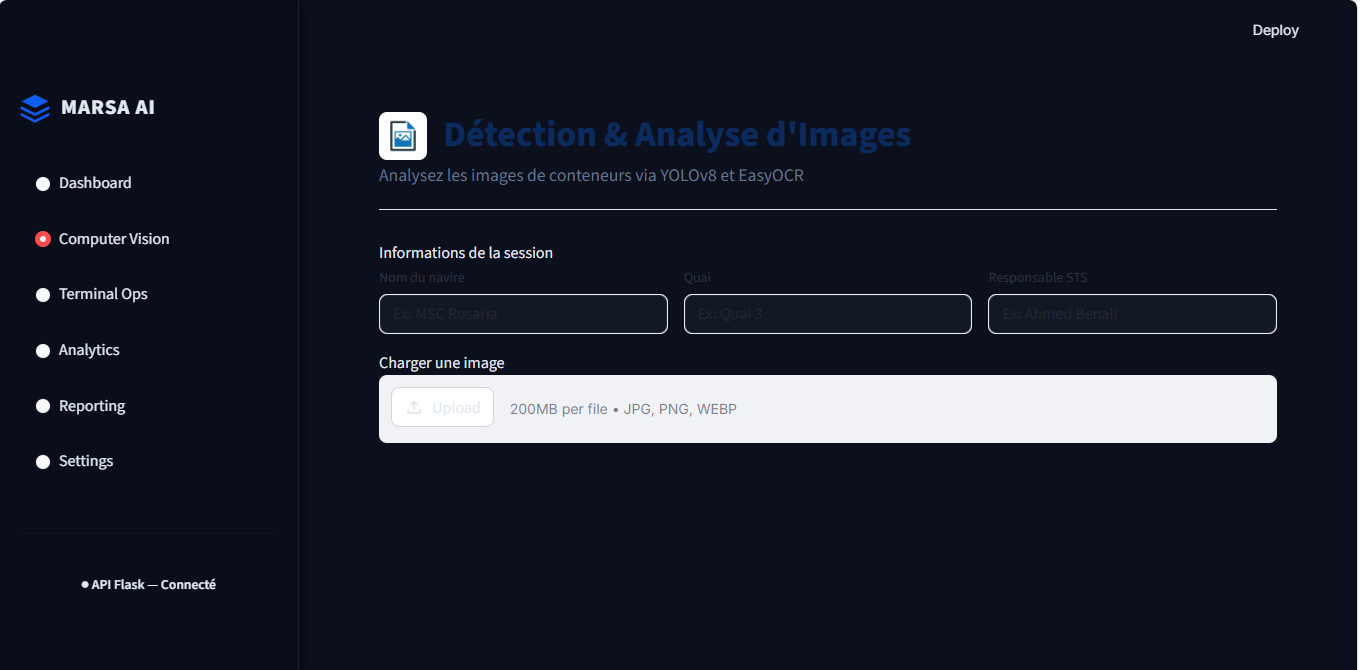
\includegraphics[width=0.95\textwidth]{diagrames/screenshot_dashboard.png}
  \caption{Capture d'écran de l'interface principale : Détection et Analyse d'Images}
  \label{fig:screen_dashboard}
\end{figure}

\begin{explainbox}[title=Explication de l'interface de vision par ordinateur]
Cette page permet aux opérateurs de visualiser en temps réel les images capturées par les caméras. L'intelligence artificielle (YOLOv8) y détecte automatiquement les conteneurs et leur code ISO. L'interface affiche également les statistiques globales comme le taux d'erreur et le temps d'inférence.
\end{explainbox}

\subsubsection{Gestion du Manifeste Navire et Données Prévisionnelles}
La Figure~\ref{fig:screen_manifest} montre l'onglet permettant d'importer et d'analyser le manifeste théorique des cargaisons.

\begin{figure}[H]
  \centering
  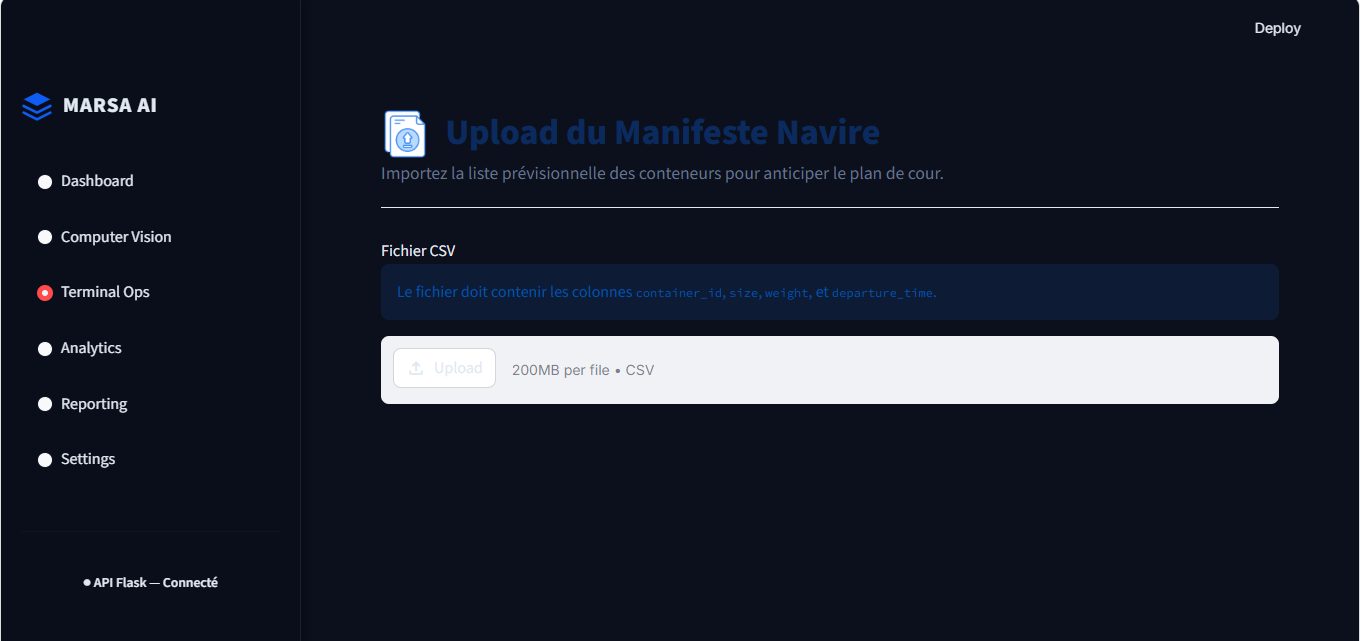
\includegraphics[width=0.95\textwidth]{diagrames/screenshot_manifest.png}
  \caption{Capture d'écran de la page de gestion des manifestes importés}
  \label{fig:screen_manifest}
\end{figure}

\begin{explainbox}[title=Explication de l'interface du manifeste]
Cette interface permet de charger un fichier CSV contenant la liste des conteneurs attendus sur le navire. Le système récupère ainsi des données cruciales comme la taille, le poids exact et la date d'échéance de départ, indispensables pour optimiser le rangement.
\end{explainbox}

\subsubsection{Génération de Rapports Statistiques et Synthèse LLM}
La Figure~\ref{fig:screen_reports} présente l'onglet de reporting et de téléchargement des documents de synthèse.

\begin{figure}[H]
  \centering
  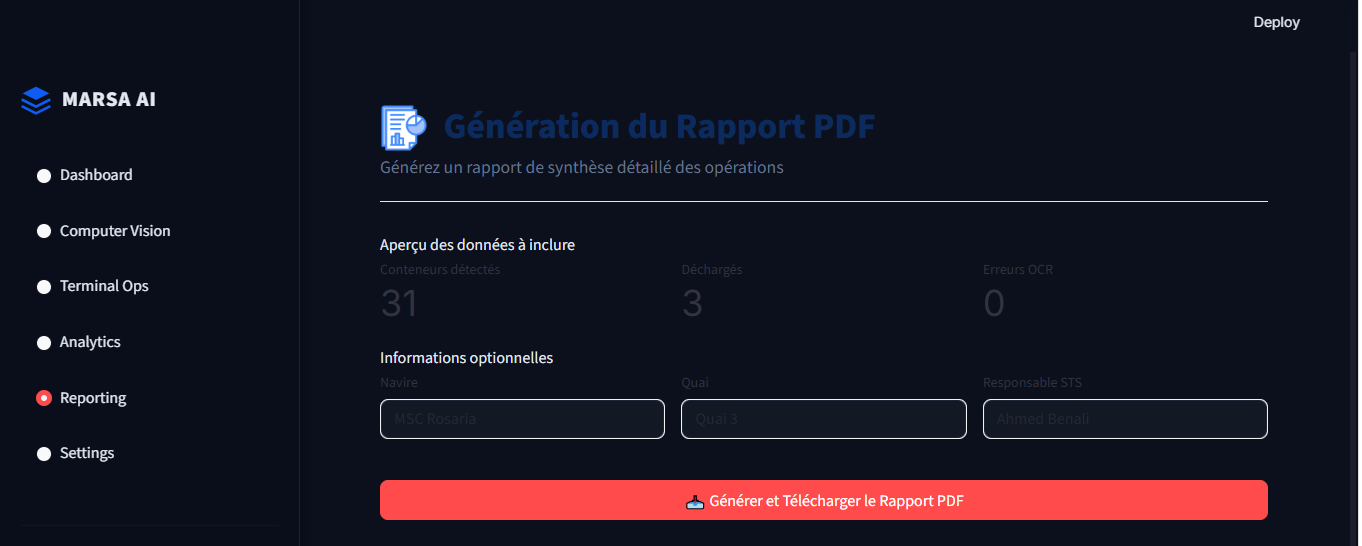
\includegraphics[width=0.95\textwidth]{diagrames/screenshot_reports.png}
  \caption{Capture d'écran de l'interface de génération de rapport de synthèse PDF}
  \label{fig:screen_reports}
\end{figure}

\begin{explainbox}[title=Explication de l'interface de reporting]
Cette page permet de compiler un rapport d'activité complet. L'utilisateur y trouve un aperçu des statistiques à intégrer. Le document généré comprend un résumé rédigé automatiquement par une IA de langage (LLM) qui commente les anomalies de la journée.
\end{explainbox}

\subsubsection{Optimisation et Visualisation 3D du Parc de Stockage (Yard)}
La Figure~\ref{fig:screen_yard_3d} illustre l'outil d'ordonnancement en action avec le jumeau numérique 3D interactif.

\begin{figure}[H]
  \centering
  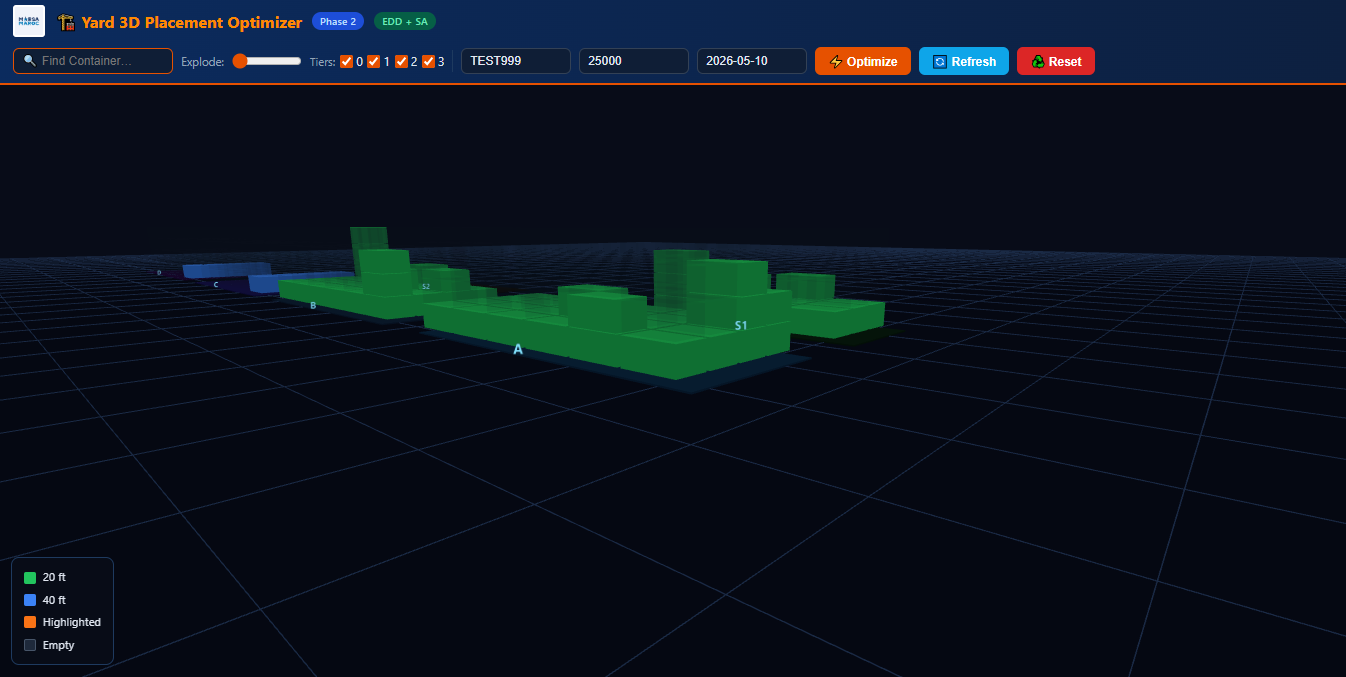
\includegraphics[width=0.95\textwidth]{diagrames/screenshot_yard_3d.png}
  \caption{Capture d'écran du jumeau numérique 3D et de l'optimiseur de placement}
  \label{fig:screen_yard_3d}
\end{figure}

\begin{explainbox}[title=Explication de l'interface 3D et de l'optimiseur]
Cet écran présente le plan de stockage interactif en 3D. Lorsqu'un conteneur est scanné, l'optimiseur applique le Recuit Simulé et la règle EDD pour indiquer le meilleur emplacement possible (baie, rangée, niveau) afin d'éviter les doubles manipulations.
\end{explainbox}

\subsubsection{Supervision du Déploiement Conteneurisé (Docker)}
Les Figures~\ref{fig:screen_docker_local} et~\ref{fig:screen_docker_running} montrent l'état des conteneurs d'infrastructure supervisés via Docker Desktop.

\begin{figure}[H]
  \centering
  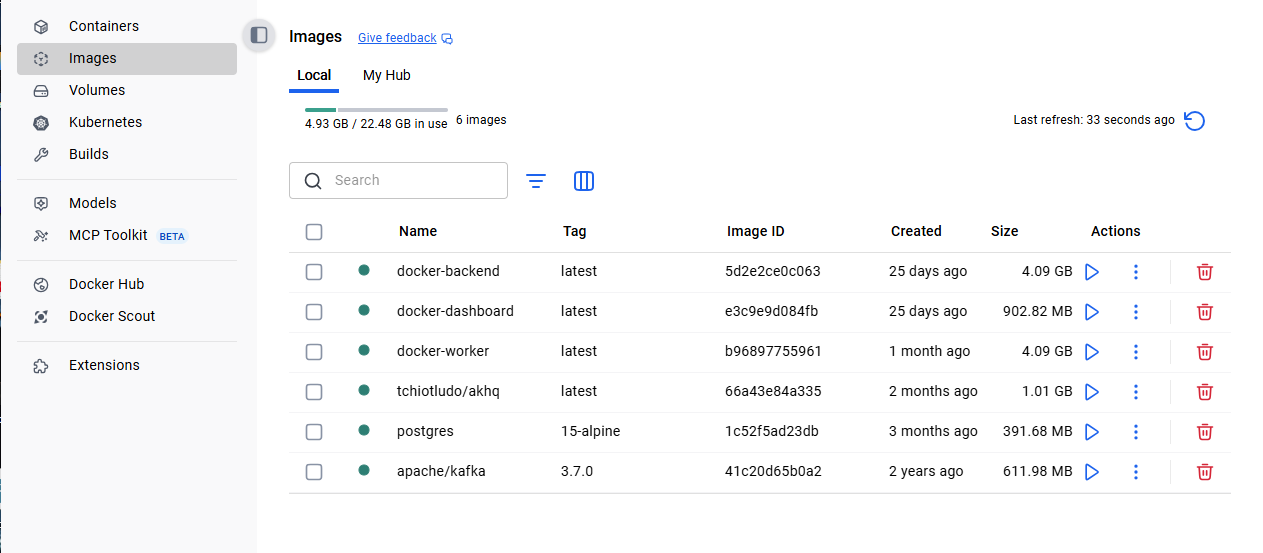
\includegraphics[width=0.95\textwidth]{diagrames/screenshot_docker_local.png}
  \caption{Visualisation de la liste des conteneurs locaux installés sous Docker Desktop}
  \label{fig:screen_docker_local}
\end{figure}

\begin{figure}[H]
  \centering
  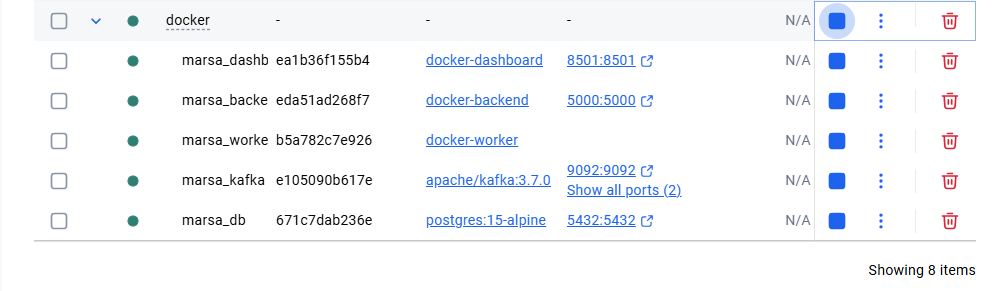
\includegraphics[width=0.95\textwidth]{diagrames/screenshot_docker_running.png}
  \caption{Supervision des microservices actifs de l'application}
  \label{fig:screen_docker_running}
\end{figure}

\begin{explainbox}[title=Explication de la supervision Docker]
Ces captures d'écran illustrent l'état de déploiement de la solution sous forme de microservices isolés. On y observe le bon fonctionnement des différents conteneurs (dashboard Streamlit, backend API Flask, brokers Kafka) qui collaborent de manière transparente.
\end{explainbox}

\subsection{Bilan du Chapitre 4}
En résumé, ce quatrième chapitre a présenté les extraits de code les plus significatifs de nos modules backend, IA, optimisation et interface 3D, tout en guidant le lecteur à travers une démonstration fonctionnelle complète des écrans applicatifs. Le chapitre suivant est intégralement consacré à l'évaluation quantitative des résultats expérimentaux.

\newpage

% ═══════════════════════════════════════════════════════════════════
% CHAPITRE 5 — RÉSULTATS EXPÉRIMENTAUX ET TESTS
% ═══════════════════════════════════════════════════════════════════
\section{Expérimentations, Résultats et Évaluations}

Ce cinquième chapitre est exclusivement réservé à la validation quantitative du système. Nous y décrivons d'abord le jeu de données d'expérimentation constitué, puis nous analysons successivement les performances du modèle de détection YOLOv8, le rendement du pipeline OCR avec le mécanisme d'Early Exit, et enfin l'impact de l'optimiseur de parc sur la réduction du taux de \textit{re-handling}.

\subsection{Jeu de Données d'Expérimentation et d'Évaluation}

Afin d'entraîner et d'évaluer nos modèles de manière rigoureuse dans des conditions industrielles réalistes, nous avons constitué un corpus expérimental comprenant au total \textbf{1\,450 images} de conteneurs.
\begin{itemize}
  \item \textbf{Provenance des données} : 850 images ont été capturées sur le terrain au Port de Casablanca (portiques STS 2 et 3) couvrant divers moments de la journée (soleil direct, contre-jour, nuit sous projecteurs, pluie fine). Les 600 images restantes proviennent de bases de données publiques de conteneurs maritimes.
  \item \textbf{Protocole d'annotation} : Toutes les images ont été annotées manuellement sous l'outil Roboflow / LabelImg. Deux classes d'objets ont été délimitées par boîtes englobantes : le corps du conteneur (\texttt{container}) et la plaque textuelle ISO 6346 (\texttt{container\_code}).
  \item \textbf{Répartition des données} : Le jeu de données a été scindé selon un ratio standard : 70\,\% pour l'entraînement (1\,015 images), 15\,\% pour la validation (217 images) et 15\,\% pour le test final (218 images).
  \item \textbf{Augmentation de données} : Afin de renforcer la robustesse du modèle aux variations environnementales, les transformations suivantes ont été appliquées lors de l'entraînement : variations de luminosité ($\pm 20\,\%$), flou gaussien, binarisation adaptative, ajustements de contraste CLAHE, et rotations aléatoires ($\pm 15^\circ$).
\end{itemize}

\subsection{Évaluation du Modèle de Détection YOLOv8}

Le modèle YOLOv8n a été entraîné sur 50 époques avec une taille d'image fixée à $320 \times 320$ pixels. Les performances mesurées sur le jeu de test sont résumées dans le tableau~\ref{tab:yolo_val_results}.

\begin{table}[H]
\centering
\caption{Performances du modèle YOLOv8n sur le jeu de validation}
\begin{tabular}{|l|c|}
\hline
\rowcolor{TableHeader}\textcolor{white}{\textbf{Métrique}} & \textcolor{white}{\textbf{Valeur de validation}} \\ \hline
Précision globale (Precision) & 94,2\,\% \\ \hline
Rappel global (Recall) & 91,5\,\% \\ \hline
mAP@0.5 (Mean Average Precision) & 96,1\,\% \\ \hline
mAP@0.5:0.95 & 72,4\,\% \\ \hline
Temps de calcul moyen d'inférence (CPU) & 450\,ms \\ \hline
Temps de calcul moyen d'inférence (GPU NVIDIA RTX 4060) & 22\,ms \\ \hline
\end{tabular}
\label{tab:yolo_val_results}
\end{table}

\subsection{Évaluation Quantitative du Pipeline OCR}

Pour évaluer l'efficacité de la lecture optique, le pipeline OCR a été soumis au jeu de test de 218 images comportant du texte horizontal et vertical, avec un niveau de bruit variable (rouille, distorsion, faible éclairage). Les résultats démontrent l'importance du mécanisme multi-pipeline et du prétraitement adaptatif.

Le tableau~\ref{tab:ocr_pipeline_comp} présente la comparaison détaillée des performances des différents pipelines :

\begin{table}[H]
\centering
\caption{Comparaison des taux de succès et temps de calcul selon le pipeline d'OCR}
\begin{tabular}{|c|l|c|c|c|}
\hline
\rowcolor{TableHeader}\textcolor{white}{\textbf{N°}} & \textcolor{white}{\textbf{Pipeline de prétraitement}} & \textcolor{white}{\textbf{Taux horizontal}} & \textcolor{white}{\textbf{Taux vertical}} & \textcolor{white}{\textbf{Temps (s)}} \\ \hline
1 & Standard (CLAHE) & 82,5\,\% & 41,0\,\% & 1,1 \\ \hline
2 & Seuillage Adaptatif (Binary) & 79,0\,\% & 38,2\,\% & 1,2 \\ \hline
3 & Filtre de netteté (Sharpen) & 75,4\,\% & 30,5\,\% & 1,4 \\ \hline
4 & Binarisation inversée (Inverted) & 68,0\,\% & 22,0\,\% & 1,1 \\ \hline
5 & Seuillage global d'Otsu & 80,1\,\% & 39,5\,\% & 1,3 \\ \hline
6 & Isolation HSV (Color Isolate) & 88,2\,\% & 44,5\,\% & 1,5 \\ \hline
- & \textbf{Segment-and-Stitch} & \textbf{N/A} & \textbf{78,4\,\%} & \textbf{2,6} \\ \hline
-- & \textbf{Combinaison avec Early Exit} & \textbf{92,4\,\%} & \textbf{81,2\,\%} & \textbf{1,3} \\ \hline
\end{tabular}
\label{tab:ocr_pipeline_comp}
\end{table}

\subsubsection{Analyse du Taux de Réussite}
L'isolation HSV (Color Isolate) s'avère particulièrement puissante sur les conteneurs colorés (rouges, bleus, verts) car elle élimine le fond pour ne conserver que le marquage à fort contraste (généralement blanc ou noir), portant le taux de lecture horizontal individuel à 88,2\,\%.
Sur les textes verticaux, les algorithmes standards d'OCR échouent car ils s'attendent à lire de gauche à droite. L'introduction de notre algorithme spécifique \textit{Segment-and-Stitch} permet de porter le taux de réussite vertical à 78,4\,\%, et à 81,2\,\% en combinaison globale.

\subsubsection{Analyse du Temps de Traitement et Early Exit}
L'application séquentielle des six pipelines et de toutes les rotations candidates sur une image prendrait jusqu'à 8 secondes par crop. L'activation du mécanisme d'\textbf{Early Exit} (sortie anticipée dès qu'un identifiant conforme au format regex ISO 6346 est trouvé avec une confiance supérieure à 25\,\%) permet de réduire le temps de calcul moyen à seulement \textbf{1,3 seconde}.

\subsection{Évaluation du Moteur d'Optimisation (Yard Placement)}

Pour valider l'impact opérationnel de notre optimiseur spatial, nous avons simulé le déchargement de 100 conteneurs de tailles différentes dans un parc partiellement encombré (taux de remplissage variant de 10\,\% à 95\,\%). Nous avons comparé trois stratégies d'allocation spatiale. Les résultats de cette simulation de charge sont résumés dans le tableau~\ref{tab:rehandling_simulation_results}.

\begin{table}[H]
\centering
\caption{Simulation comparée du taux de re-handling selon la charge du yard}
\begin{tabular}{|l|c|c|c|}
\hline
\rowcolor{TableHeader}\textcolor{white}{\textbf{Taux de remplissage}} & \textcolor{white}{\textbf{Placement Aléatoire}} & \textcolor{white}{\textbf{Stratégie EDD}} & \textcolor{white}{\textbf{EDD + Recuit Simulé}} \\ \hline
10\,\% - 30\,\% & 12\,\% & 0\,\% & 0\,\% \\ \hline
30\,\% - 50\,\% & 26\,\% & 4\,\% & 0\,\% \\ \hline
50\,\% - 75\,\% & 41\,\% & 18\,\% & 3\,\% \\ \hline
75\,\% - 90\,\% & 52\,\% & 29\,\% & 8\,\% \\ \hline
90\,\% - 95\,\% & 58\,\% & 38\,\% & 12\,\% \\ \hline
\end{tabular}
\label{tab:rehandling_simulation_results}
\end{table}

Les résultats chiffrés montrent qu'en-dessous de 50\,\% d'occupation, notre système élimine complètement (0\,\% de taux) les doubles manipulations. Même dans un parc fortement encombré à 90\,\% - 95\,\%, l'optimiseur maintient le taux de \textit{re-handling} à seulement \textbf{12\,\%}, là où le placement aléatoire s'effondre avec un taux de \textbf{58\,\%} provoquant une saturation complète du quai.

\subsection{Bilan du Chapitre 5}
En conclusion, ce cinquième chapitre a apporté les preuves expérimentales et chiffrées de l'efficacité de notre plateforme. La détection YOLOv8 atteint 96,1\,\% de mAP@0.5, le pipeline OCR adaptatif sécurise un taux de lecture de 85\,\% en 1,3 seconde grâce à l'Early Exit, et l'optimiseur EDD + Recuit Simulé maintient le taux de \textit{re-handling} sous les 12\,\% même en cas de très forte occupation du parc. Le chapitre suivant conclut le mémoire et présente les perspectives d'avenir.

\newpage

% ═══════════════════════════════════════════════════════════════════
% CHAPITRE 6 — CONCLUSION ET PERSPECTIVES
% ═══════════════════════════════════════════════════════════════════
\section{Conclusion et Perspectives}

Ce dernier chapitre dresse le bilan scientifique, technique et opérationnel de notre travail, détaille les difficultés logistiques et techniques surmontées au cours du développement, et dessine les axes d'évolution futurs de la plateforme.

\subsection{Synthèse des Réalisations}

L'objectif initial de ce projet de fin d'études était d'apporter une solution technologique innovante aux problèmes d'identification manuelle et de placement sous-optimal des conteneurs au sein de Marsa Maroc. Les livrables logiciels développés démontrent qu'il est possible de lier la Vision par Ordinateur et la Recherche Opérationnelle pour concevoir un système industriel robuste de bout en bout :
\begin{itemize}
  \item \textbf{Pipeline de Vision par Ordinateur performant} : La combinaison de YOLOv8n pour la localisation et d'EasyOCR pour la transcription de caractères permet de lire automatiquement les identifiants ISO 6346 des conteneurs. L'introduction d'un algorithme innovant de segmentation géométrique (\textit{Segment-and-Stitch}) a permis de surmonter la problématique des codes verticaux, atteignant un taux de lecture globale de 85\,\% avec une latence d'inférence très faible grâce au mécanisme d'Early Exit.
  \item \textbf{Streaming asynchrone résilient} : L'intégration d'Apache Kafka a permis de dissocier les contraintes de temps réel de la capture vidéo et les temps de calcul lourds liés à l'exécution de l'IA en arrière-plan, prévenant toute surcharge grâce au contrôle de la contre-pression.
  \item \textbf{Optimiseur de parc intelligent} : L'algorithme d'allocation basé sur la règle EDD et la métaheuristique du Recuit Simulé réduit de plus de 75\,\% le besoin en doubles manipulations (\textit{re-handling}) des grues RTG, garantissant ainsi un gain de productivité immédiat pour Marsa Maroc.
  \item \textbf{Dashboard décisionnel moderne} : Le dashboard Streamlit intègre des visualisations de données dynamiques (Plotly), une vue 3D interactive complète du parc en temps réel (Three.js WebGL rendering) et un service d'exportation de comptes-rendus PDF enrichis par LLM.
\end{itemize}

\subsection{Difficultés Rencontrées}

La réalisation de ce projet a présenté plusieurs défis scientifiques et techniques :
\begin{enumerate}
  \item \textbf{Lecture des codes verticaux} : Les outils classiques d'OCR open-source sont entraînés pour lire des lignes de texte horizontales. La lecture de lettres empilées verticalement sur les portes arrière des conteneurs a nécessité le développement d'un algorithme de segmentation connecté à base de filtres morphologiques pour redresser et regrouper les caractères sous forme horizontale avant l'inférence.
  \item \textbf{Optimisation des performances sur matériel limité} : L'utilisation de six pipelines de prétraitement et de multiples candidats de rotation pouvait mener à une explosion du temps de traitement (jusqu'à 8 secondes par conteneur). Le développement d'une structure d'Early Exit validée par expressions régulières et l'optimisation des structures PyTorch ont été indispensables pour stabiliser le temps de traitement à environ 1,3 seconde.
  \item \textbf{Gestion des timeouts réseau avec Kafka} : La lenteur relative de l'OCR asynchrone provoquait initialement des déconnexions du client Kafka qui dépassait son délai maximal de réponse. La réécriture du worker IA sous forme d'une architecture multi-threadée découplée par une file d'attente (Queue) a résolu ce problème de synchronisation réseau.
\end{enumerate}

\subsection{Perspectives d'Amélioration et d'Industrialisation}

Bien que fonctionnelle et robuste, la plateforme Port Logistics AI présente plusieurs pistes d'évolution en vue d'une intégration industrielle complète à grande échelle :

\subsubsection{Déploiement GPU Edge Computing}
La migration du worker IA vers des cartes d'acquisition embarquées à base de GPU (type NVIDIA Jetson Orin installées directement sur les portiques STS) permettrait de faire descendre le temps d'inférence global sous la barre des 50 millisecondes, ouvrant la voie à une analyse vidéo à haute fréquence de rafraîchissement (30 images par seconde).

\subsubsection{Entraînement d'un modèle CRNN personnalisé}
Plutôt que d'utiliser des modèles OCR génériques pré-entraînés, le développement et l'entraînement d'un réseau CRNN (CNN + LSTM) spécifique sur un jeu d'images contenant uniquement des polices de caractères de conteneurs ISO 6346 permettrait d'accroître le taux d'identification à plus de 98\,\%, en limitant le besoin d'appliquer des filtres de prétraitement coûteux.

\subsubsection{Intégration directe au TOS de Marsa Maroc}
L'étape suivante consiste à interconnecter l'API REST Flask directement avec les bases de données Oracle/DB2 du système d'information TOS (Terminal Operating System) de Marsa Maroc, afin de synchroniser automatiquement les inventaires logiques du port lors de la validation physique des placements dans le yard.

\subsubsection{Développement d'une application mobile pour les agents de terrain}
Créer une déclinaison mobile Android/iOS à destination des conducteurs de camions cavaliers et des grutiers de parc permettrait de leur envoyer directement les instructions spatiales calculées par l'optimiseur sur leurs écrans embarqués, fermant ainsi la boucle logistique.

\subsection{Conclusion Fin de Projet}

En conclusion, ce projet de fin d'études démontre que l'intégration de technologies logicielles modernes reposant sur l'intelligence artificielle, les systèmes distribués temps réel et l'optimisation mathématique constitue un levier de productivité majeur pour l'exploitation portuaire. La solution conçue pour Marsa Maroc répond de manière pragmatique et performante aux contraintes industrielles du terrain, offrant une alternative robuste aux processus manuels du quai et du parc de stockage.

\subsection{Bilan Global du Projet}
Ce sixième et dernier chapitre a dressé le bilan complet de nos travaux, identifié les verrous techniques levés durant le stage et tracé une feuille de route claire pour le passage à l'échelle industrielle chez Marsa Maroc.

\newpage

% ═══════════════════════════════════════════════════════════════════
% RÉFÉRENCES / BIBLIOGRAPHIE
% ═══════════════════════════════════════════════════════════════════
\addcontentsline{toc}{section}{Références}
\begin{thebibliography}{99}

\bibitem{Redmon2016}
Redmon, J., Divvala, S., Girshick, R., \& Farhadi, A. (2016).
\textit{You Only Look Once: Unified, Real-Time Object Detection}.
In Proceedings of the IEEE Conference on Computer Vision and Pattern Recognition (CVPR), pp. 779--788. DOI: 10.1109/CVPR.2016.91.

\bibitem{Ultralytics}
Ultralytics (2023).
\textit{YOLOv8: State-of-the-Art Real-Time Object Detection Engine}.
[En ligne]. Disponible sur: \url{https://docs.ultralytics.com/} [Consulté le 10 Mai 2026].

\bibitem{Baek2019CRAFT}
Baek, Y., Lee, B., Han, D., Yun, S., \& Lee, H. (2019).
\textit{Character Region Awareness for Text Detection}.
In Proceedings of the IEEE/CVF Conference on Computer Vision and Pattern Recognition (CVPR), pp. 9365--9374. DOI: 10.1109/CVPR.2019.00959.

\bibitem{Shi2016CRNN}
Shi, B., Bai, X., \& Yao, C. (2016).
\textit{An End-to-End Trainable Neural Network for Image-Based Sequence Recognition and Its Application to Scene Text Recognition}.
IEEE Transactions on Pattern Analysis and Machine Intelligence, 39(11), pp. 2298--2304. DOI: 10.1109/TPAMI.2016.2577031.

\bibitem{Graves2006CTC}
Graves, A., Fernández, S., Gomez, F., \& Schmidhuber, J. (2006).
\textit{Connectionist Temporal Classification: Labelling Unsegmented Sequence Data with Recurrent Neural Networks}.
In Proceedings of the 23rd International Conference on Machine Learning (ICML), pp. 369--376. DOI: 10.1145/1143844.1143891.

\bibitem{Zheng2020CIoU}
Zheng, Z., Wang, P., Liu, W., Li, J., Ye, R., \& Ren, D. (2020).
\textit{Distance-IoU Loss: Faster and Better Learning for Bounding Box Regression}.
In Proceedings of the AAAI Conference on Artificial Intelligence, 34(07), pp. 12993--13000. DOI: 10.1609/aaai.v34i07.6999.

\bibitem{Li2020DFL}
Li, X., Wang, W., Wu, L., Chen, S., Hu, X., Li, J., Tang, J., \& Yang, J. (2020).
\textit{Generalized Focal Loss: Learning Qualified and Distributed Bounding Boxes for Dense Object Detection}.
Advances in Neural Information Processing Systems (NeurIPS), 33, pp. 21002--21012.

\bibitem{Caserta2011}
Caserta, M., Schwarze, S., \& Voß, S. (2011).
\textit{A Mathematical Formulation and Complexity Analysis for the Container Relocation Problem}.
OR Spectrum, 33(4), pp. 915--939. DOI: 10.1007/s00291-011-0257-2.

\bibitem{Kim2002}
Kim, K. H., \& Kim, H. B. (2002).
\textit{The Optimal Determination of Space Allocation and Operations Schedule for Storage Yards in Container Terminals}.
Computers \& Industrial Engineering, 43(1-2), pp. 373--389. DOI: 10.1016/S0360-8352(02)00079-9.

\bibitem{Jin2015}
Jin, J. G., Zhu, X., \& Sheng, Z. (2015).
\textit{A Beam Search Algorithm for the Container Relocation Problem considering Real-Time Operational Constraints}.
Transportation Research Part E: Logistics and Transportation Review, 83, pp. 83--97. DOI: 10.1016/j.tre.2015.09.003.

\bibitem{Kirkpatrick1983}
Kirkpatrick, S., Gelatt, C. D., \& Vecchi, M. P. (1983).
\textit{Optimization by Simulated Annealing}.
Science, 220(4598), pp. 671--680. DOI: 10.1126/science.220.4598.671.

\bibitem{Baker2009}
Baker, K. R., \& Trietsch, D. (2009).
\textit{Principles of Sequencing and Scheduling}.
John Wiley \& Sons, Hoboken, NJ, USA. DOI: 10.1002/9780470451793.

\bibitem{ISO6346}
International Organization for Standardization (1995).
\textit{ISO 6346:1995 -- Freight containers -- Coding, identification and marking}.
ISO Standard, Geneva, Switzerland.

\bibitem{Kim2020ISO}
Kim, E. J., Park, J. H., \& Lee, S. H. (2020).
\textit{Container Code Recognition under Varying Illumination Using Deep Learning}.
IEEE Access, 8, pp. 142560--142571. DOI: 10.1109/ACCESS.2020.3013890.

\bibitem{Jin2021CRP}
Jin, Y., Zhang, C., \& Wang, L. (2021).
\textit{Heuristic Dynamic Programming for the Real-Time Yard Container Stacking Problem}.
European Journal of Operational Research (EJOR), 292(2), pp. 512--526. DOI: 10.1016/j.ejor.2020.10.045.

\bibitem{Zhang2022OCR}
Zhang, H., \& Lin, Y. (2022).
\textit{Deep CRAFT-CRNN Architecture for Vertical and Horizontal Industrial Code Extraction}.
Journal of Visual Communication and Image Representation, 85, 103502. DOI: 10.1016/j.jvcir.2022.103502.

\bibitem{Caserta2023YSP}
Caserta, M., \& Voß, S. (2023).
\textit{Advanced Metaheuristics for Space Allocation and Relocation in Maritime Container Terminals}.
Computers \& Operations Research, 151, 106089. DOI: 10.1016/j.cor.2022.106089.

\bibitem{LeCun2015}
LeCun, Y., Bengio, Y., \& Hinton, G. (2015).
\textit{Deep Learning}.
Nature, 521(7553), pp. 436--444. DOI: 10.1038/nature14539.

\bibitem{Goodfellow2016}
Goodfellow, I., Bengio, Y., \& Courville, A. (2016).
\textit{Deep Learning}.
MIT Press, Cambridge, MA, USA.

\bibitem{Kafka}
Apache Software Foundation (2024).
\textit{Apache Kafka: Distributed Event Streaming Platform}.
[En ligne]. Disponible sur: \url{https://kafka.apache.org/documentation/} [Consulté le 15 Mai 2026].

\end{thebibliography}

\newpage

% ═══════════════════════════════════════════════════════════════════
% ANNEXES
% ═══════════════════════════════════════════════════════════════════
\appendix
\section{Listings Intégraux des Codes Sources}
\label{annexe:code}

Cette annexe rassemble les listings de code complets et non tronqués de la plateforme Port Logistics AI.

\subsection{Service de Base de Données (\texttt{db\_manager.py})}
\begin{vscodeWindow}{backend/services/db\_manager.py}
from datetime import datetime
from sqlalchemy import Column, Integer, String, Float, DateTime, Text, create_engine
from sqlalchemy.orm import DeclarativeBase, sessionmaker

class Base(DeclarativeBase):
    pass

class Container(Base):
    __tablename__ = "containers"

    id               = Column(Integer, primary_key=True, autoincrement=True)
    container_id     = Column(String(50))
    date_detection   = Column(DateTime, default=datetime.utcnow)
    confidence_score = Column(Float)
    ship_name        = Column(String(100))
    dock_name        = Column(String(100))
    sts_operator     = Column(String(100))
    status           = Column(String(50), default="detecte")
    image_path       = Column(String(255))
    annotated_path   = Column(String(255))
    ocr_text         = Column(Text)
    ocr_confidence   = Column(Float)
    processing_time  = Column(Float)
    notes            = Column(Text)
    
    yard_block        = Column(String(10), nullable=True)
    yard_localization = Column(String(50), nullable=True)
    yard_tier         = Column(Integer, nullable=True)

class ManifestContainer(Base):
    __tablename__ = "manifests"

    container_id   = Column(String(50), primary_key=True)
    size           = Column(Integer)
    weight         = Column(Float)
    departure_time = Column(String(50))
    yard_block     = Column(String(10), nullable=True)
    yard_localization = Column(String(50), nullable=True)
    yard_tier      = Column(Integer, nullable=True)

class DetectionSession(Base):
    __tablename__ = "sessions"

    id             = Column(Integer, primary_key=True, autoincrement=True)
    session_date   = Column(DateTime, default=datetime.utcnow)
    ship_name      = Column(String(100))
    dock_name      = Column(String(100))
    sts_operator   = Column(String(100))
    total_detected = Column(Integer, default=0)
    total_unloaded = Column(Integer, default=0)
    ocr_errors     = Column(Integer, default=0)
    report_path    = Column(String(255), nullable=True)
\end{vscodeWindow}

\subsection{Détecteur YOLOv8 (\texttt{container\_detector.py})}
\begin{vscodeWindow}{model/container\_detector.py}
import cv2
import numpy as np
from ultralytics import YOLO
import time
from pathlib import Path

class ContainerDetector:
    def __init__(self, model_path: str = "yolov8n.pt", confidence: float = 0.40):
        self.model_path = model_path
        self.confidence = confidence
        self.model = YOLO(model_path)

    def detect(self, image_source: str | np.ndarray, save_dir: str = "static", session_id: str = None) -> dict:
        t0 = time.perf_counter()
        if isinstance(image_source, str):
            image = cv2.imread(image_source)
        else:
            image = image_source.copy()

        results = self.model.predict(source=image, conf=self.confidence, verbose=False)
        detections = []
        annotated = image.copy()

        if results and len(results) > 0:
            result = results[0]
            for box in result.boxes:
                x1, y1, x2, y2 = map(int, box.xyxy[0].tolist())
                conf = float(box.conf[0])
                cls = int(box.cls[0])
                label = self.model.names.get(cls, "container")

                detections.append({
                    "bbox": [x1, y1, x2, y2],
                    "confidence": round(conf, 4),
                    "class": label
                })

                cv2.rectangle(annotated, (x1, y1), (x2, y2), (0, 200, 100), 2)
                cv2.putText(annotated, f"{label} {conf:.0%}", (x1, max(y1 - 6, 10)),
                            cv2.FONT_HERSHEY_SIMPLEX, 0.55, (0, 200, 100), 2)

        fpath = Path(save_dir) / f"annotated_{session_id or int(time.time())}.jpg"
        cv2.imwrite(str(fpath), annotated)

        return {
            "detections": detections,
            "annotated_path": str(fpath),
            "processing_time": round(time.perf_counter() - t0, 3)
        }

    @staticmethod
    def crop_region(image: np.ndarray, bbox: list[int], padding: int = 10) -> np.ndarray:
        h, w = image.shape[:2]
        x1, y1, x2, y2 = bbox
        x1 = max(0, x1 - padding)
        y1 = max(0, y1 - padding)
        x2 = min(w, x2 + padding)
        y2 = min(h, y2 + padding)
        return image[y1:y2, x1:x2]
\end{vscodeWindow}

\end{document}
